%% For double-blind review submission, w/o CCS and ACM Reference (max submission space)
\documentclass[acmsmall,review,anonymous]{acmart}\settopmatter{printfolios=true,printccs=false,printacmref=false}


%% Journal information
%% Supplied to authors by publisher for camera-ready submission;
%% use defaults for review submission.
\acmJournal{PACMPL}
\acmVolume{1}
\acmNumber{CONF} % CONF = POPL or ICFP or OOPSLA
\acmArticle{1}
\acmYear{2018}
\acmMonth{1}
\acmDOI{} % \acmDOI{10.1145/nnnnnnn.nnnnnnn}
\startPage{1}

%% Copyright information
%% Supplied to authors (based on authors' rights management selection;
%% see authors.acm.org) by publisher for camera-ready submission;
%% use 'none' for review submission.
\setcopyright{none}
%\setcopyright{acmcopyright}
%\setcopyright{acmlicensed}
%\setcopyright{rightsretained}
%\copyrightyear{2018}           %% If different from \acmYear

%% Bibliography style
\bibliographystyle{ACM-Reference-Format}
%% Citation style
%% Note: author/year citations are required for papers published as an
%% issue of PACMPL.
\citestyle{acmauthoryear}   %% For author/year citations


%%%%%%%%%%%%%%%%%%%%%%%%%%%%%%%%%%%%%%%%%%%%%%%%%%%%%%%%%%%%%%%%%%%%%%
%% Note: Authors migrating a paper from PACMPL format to traditional
%% SIGPLAN proceedings format must update the '\documentclass' and
%% topmatter commands above; see 'acmart-sigplanproc-template.tex'.
%%%%%%%%%%%%%%%%%%%%%%%%%%%%%%%%%%%%%%%%%%%%%%%%%%%%%%%%%%%%%%%%%%%%%%


%% Some recommended packages.
\usepackage{booktabs}   %% For formal tables:
                        %% http://ctan.org/pkg/booktabs
\usepackage{subcaption} %% For complex figures with subfigures/subcaptions
                        %% http://ctan.org/pkg/subcaption


\begin{document}

%% Title information
\title{Delta Logics: Logics for Change}         %% [Short Title] is optional;
                                        %% when present, will be used in
                                        %% header instead of Full Title.
%\titlenote{with title note}             %% \titlenote is optional;
                                        %% can be repeated if necessary;
                                        %% contents suppressed with 'anonymous'
%\subtitle{Subtitle}                     %% \subtitle is optional
%\subtitlenote{with subtitle note}       %% \subtitlenote is optional;
                                        %% can be repeated if necessary;
                                        %% contents suppressed with 'anonymous'


%% Author information
%% Contents and number of authors suppressed with 'anonymous'.
%% Each author should be introduced by \author, followed by
%% \authornote (optional), \orcid (optional), \affiliation, and
%% \email.
%% An author may have multiple affiliations and/or emails; repeat the
%% appropriate command.
%% Many elements are not rendered, but should be provided for metadata
%% extraction tools.

%% Author with single affiliation.
\author{First1 Last1}
\authornote{with author1 note}          %% \authornote is optional;
                                        %% can be repeated if necessary
\orcid{nnnn-nnnn-nnnn-nnnn}             %% \orcid is optional
\affiliation{
  \position{Position1}
  \department{Department1}              %% \department is recommended
  \institution{Institution1}            %% \institution is required
  \streetaddress{Street1 Address1}
  \city{City1}
  \state{State1}
  \postcode{Post-Code1}
  \country{Country1}                    %% \country is recommended
}
\email{first1.last1@inst1.edu}          %% \email is recommended

%% Author with two affiliations and emails.
\author{First2 Last2}
\authornote{with author2 note}          %% \authornote is optional;
                                        %% can be repeated if necessary
\orcid{nnnn-nnnn-nnnn-nnnn}             %% \orcid is optional
\affiliation{
  \position{Position2a}
  \department{Department2a}             %% \department is recommended
  \institution{Institution2a}           %% \institution is required
  \streetaddress{Street2a Address2a}
  \city{City2a}
  \state{State2a}
  \postcode{Post-Code2a}
  \country{Country2a}                   %% \country is recommended
}
\email{first2.last2@inst2a.com}         %% \email is recommended
\affiliation{
  \position{Position2b}
  \department{Department2b}             %% \department is recommended
  \institution{Institution2b}           %% \institution is required
  \streetaddress{Street3b Address2b}
  \city{City2b}
  \state{State2b}
  \postcode{Post-Code2b}
  \country{Country2b}                   %% \country is recommended
}
\email{first2.last2@inst2b.org}         %% \email is recommended


%% Abstract
%% Note: \begin{abstract}...\end{abstract} environment must come
%% before \maketitle command
\begin{abstract}
We define delta logics, a new class of logics designed to express verification conditions
of basic blocks that destructively manipulate a heap. Delta logic describes separately the part of the heap that changes
and its unchanged context. Utilizing this simplicity and separation, we develop an expressive decidable
delta logic that states properties of lists using a variety of measures on them, including their heaplets, 
their length, the multiset of keys stored in them, the min/max keys stored in them, and their sortedness. We show that 
delta logics and the associated decision procedure yield a practically viable verification engine through an 
implementation of the technique and an evaluation of it.
\end{abstract}


%% 2012 ACM Computing Classification System (CSS) concepts
%% Generate at 'http://dl.acm.org/ccs/ccs.cfm'.
\begin{CCSXML}
<ccs2012>
<concept>
<concept_id>10011007.10011006.10011008</concept_id>
<concept_desc>Software and its engineering~General programming languages</concept_desc>
<concept_significance>500</concept_significance>
</concept>
<concept>
<concept_id>10003456.10003457.10003521.10003525</concept_id>
<concept_desc>Social and professional topics~History of programming languages</concept_desc>
<concept_significance>300</concept_significance>
</concept>
</ccs2012>
\end{CCSXML}

\ccsdesc[500]{Software and its engineering~General programming languages}
\ccsdesc[300]{Social and professional topics~History of programming languages}
%% End of generated code


%% Keywords
%% comma separated list
\keywords{keyword1, keyword2, keyword3}  %% \keywords are mandatory in final camera-ready submission


\newcommand{\HLS}{\textit{HLS}}
\newcommand{\sem}[1]{\llbracket #1 \rrbracket}
\newcommand{\vect}[1]{\overline{#1}}

%% \maketitle
%% Note: \maketitle command must come after title commands, author
%% commands, abstract environment, Computing Classification System
%% environment and commands, and keywords command.
\maketitle

\section{Introduction}
\label{sec:intro}

Classical logics, such as first-order logic with least fixpoints or higher order logics, are often static in the sense that formulae 
describe the state of a single world. 
Verification conditions of imperative programs describe typically at least two different worlds: the pre-state
and the post-state of a program. Consequently, expressing validity of verification conditions (VCs)
naturally involves the challenge of expressing the evolving worlds of program states in a static logic.
The classical notion of strongest postcondition for programs with scalar variables does precisely this--- 
it expresses the precondition, the intermediate states of the program, and the post-state using \emph{auxiliary} 
first-order variables that capture the scalar variables at these states. The weakest precondition, again for
programs with scalar variables, solves the same problem.

The focus of this paper is in generating logical formulations of verification conditions for program snippets that manipulate the heap. The pre- and post-conditions are written in quantifier-free FO + \textit{lfp}. A lot of complex and interesting properties of heap manipulating programs can be expressed using recursively defined functions and predicates, such as `$x$ points to a linked list segment ending at $z$', `the maximum element stored in the list pointed to by $x$'. In this setting, the heap consists, minimally, of a set of pointer fields that are modeled by \emph{first-order
functions}, and the program's execution alters these functions.
Consequently, the translation of Hoare triples to validity of verification conditions is considerably harder, in comparison with programs with only scalar variables. This is further complicated by the presence of recursively defined functions/predicates that refer to data fields, which can express complex properties combining both shape and data on the heap.

There are two general ways of translating Hoare triples to verification conditions in this setting. The first is to accurately capture the Hoare triple; this typically involves two versions of the recursive functions, one for the pre-state and one for the post-state, where the two are parameterized by different sets of pointer fields. Furthermore, the verification conditions introduces quantification to precisely capture the heaplet that is changed by the program snippet. All of this makes automated reasoning of the verification condition extremely complex.

The second way is to model the heap change as an arbitrary change of the modified portion of the heap, and use \emph{frame reasoning} to argue properties are conserved across the heap transformation. This is at the heart of the design of separation logic. However, frame reasoning alone is not complete. 

For program snippets that involve function calls, we believe that frame reasoning is appropriate, and continue recommending it. However, for program snippets without function calls, we argue in this paper that an accurate encoding of the verification condition is possible that is also amenable to automated reasoning.


%However, traditional ways of reducing validation of verification conditions to logic embed the verification in logics that have much
%more expressive power than necessary, and harder to reason with; we think it is a reduction from an easier problem to a harder problem!


%\textbf{SOMETHING ABOUT FRAME REASONING}

In this paper, we identify a new class of logics called \emph{Delta-logics} for expressing verification conditions that addresses the above problem.
Formulae in delta-logics are Boolean combinations of two kinds of formulae: one, \emph{delta-specific} formulae, talk about the modified portion of the global heap, which we call $\Delta$, without using any recursive definitions; the other 
kind, called \emph{contextual/context-logic} formulae, strictly talk about the unbounded portion excluding $\Delta$, and uses recursive definitions. A set of first-order interface variables (called \emph{parameters}) are used to communicate information between $\Delta$ and the rest of the heap.

We motivate the desirable aspects of delta-logics for expressing verification conditions, and provide an overview of the mechanism of VC generation using delta-logics in  Section~\ref{sec:motivation}. 

When translating Hoare triples to VCs in delta-logic, the program snippets translate naturally
as delta-logic clearly delineates the modified heaplet from its context, and the program's transformation is a delta-specific formula. 
A technical challenge, however, is to express the pre- and post-conditions which are on both the modified and unmodified portions of the heap.
We prove a key theorem, called the \emph{Separability Theorem} that shows that any quantifier-free FO formula with recursive definitions can be expressed in delta-logics, i.e., as a boolean combination of delta-specific formulae and contextual formulae. We shall see that this separation is nontrivial, and requires the definition of new parameterized recursive functions called \emph{ranks} for each parameterized recursive definition.


%Lastly, we show how to generate VCs for such basic blocks using the separability theorem in Section~\ref{sec:VC2Delta}.

The simplicity of expressing VCs in delta logics enables us to design powerful \emph{decidable} program logics.
We define a delta-logic that expresses
properties of list segments along with a varied collection of of measures on them, including their heaplets (for expressing separation properties), 
their lengths, the multisets of keys stored in them, the min/max keys stored in them, and their sortedness. 
We show that these delta-logic formulae can be translated to equisatisfiable quantifier-free formulae \emph{without} recursive definitions. This leads us to a decision procedure for delta-logics for linked lists with all the six measures above. To the best of our knowledge, this is the most expressive decidable program logic for list manipulating programs. 

We emphasize that though delta logics 
are particularly meant for program snippets 
that do not involve function calls, we show that it
can be seamlessly combined with frame reasoning for
function calls, leading us to define a comprehensive verification technique for programs
with function calls.

Finally, we implement and evaluate our technique by expressing VCs using delta-logics and validating them using our decision procedure on a suite of programs, and show it to be effective both for verifying correct
programs and finding bugs in incorrect ones.

\medskip
\noindent
The main contributions of this paper are:
\begin{itemize}
\item A new class of logics called Delta-Logics, which are specially suited to expressing verification conditions of program manipulating a bounded set of locations.

\item A nontrivial \emph{Separability Theorem} that shows that quantifier-free FO+\textit{lfp} formulae can be translated into delta-logic formulae.

\item A technique for expressing verification conditions, of programs manipulating, heaps in delta-logics.

\item A powerful decidable delta-logic over lists and list-measures using a reduction to standard SMT theories.

\item An extension of the VC generation technique to incorporate frame reasoning for function calls with delta-logics, and consequently a decidability result for VCs of list-manipulating programs with function calls.

\item An implementation and evaluation of the VC generation and decision procedure for the delta-logic of lists and measures, showing their efficacy on a suite of list-manipulating programs, both correct programs and faulty programs.
\end{itemize}

\medskip
\noindent
The paper is organized as follows. In Section~\ref{sec:motivation}, we motivate delta-logics, the separability theorem, an overview of VC generation using delta-logics, through an illustrative example. In Section~\ref{sec:delta-logics} we formally define delta-logics and in Section~\ref{sec:separability} we prove the separability theorem. Section~\ref{sec:VC2Delta} discusses the VC generation mechanism for delta-logics from Hoare triples for basic blocks without function calls. In Section~\ref{sec:decidability} we define the decidable delta-logic of lists and list-measures and provide its decision procedure. Combined with the VC generation technique, this provides a decision procedure for the program logic of list-manipulating programs without function calls. In Section~\ref{sec:generalvc} we extend the VC generation technique to verify list-manipulating programs with function calls by incorporating frame-reasoning for function calls with delta-logics. In Section~\ref{sec:experiments} we discuss the implementation and evaluation of our technique on a suite of list-manipulating programs. Finally, in Section~\ref{sec:relwork} we discuss and compare our work with existing literature. We then conclude in Section~\ref{sec:conclusion} with some comments on future work.

\section{Overview and motivating example}
\label{sec:motivation}

In this section, we shall provide the motivation for our paper, an overview of our technique, and illustrate the method on a motivating example.

\subsection{Motivation: frame reasoning, delta changes and verification conditions}
In this part we shall describe the need for a new logic for expressing verification conditions for Hoare triples involving snippets of code that modify a bounded set of heap locations.

Let us consider a set of pointer fields $\vect{p}$ and a recursive definition of a unary predicate or function $R(x)$ defined
using least fixpoints over $\vect{p}$. Typical functions include properties such as 
``$x$ points to a linked list segment ending at the location $z$'', ``the length of the list pointed to by $x$'', 
``$x$ points to a binary search tree'', ``the set of keys stored in the tree pointed to by $x$'', ``the heaplet defined
by the tree pointed to by $x$'', etc.
Consider a Hoare triple of the form $\textit{@pre}(\vect{x}, \vect{p}, R) ~S~ \textit{@post}(\vect{x}, \vect{p}, R)$; the pre and postconditions use the recursively defined predicate/function $R$.

One simple approach is to capture the precondition using logic and use the \emph{frame rule} to reason soundly
(but incompletely) about the post-state--- i.e., we can simply ignore the definition of $R$
on the transformed heap and infer that $R(x)$ holds in the post-state if it held in the pre-state and 
the modified portion of the heap did not intersect with the underlying heaplet of $R(x)$.
This is, in practice, a very \emph{convenient and simple} reasoning that often works and is one of the foundational ideas that separation logic facilitates~\cite{Reynolds2002}. However, vanilla frame reasoning can be incomplete, as we shall argue through a motivating example (see Section~\ref{sec:motivating_example}). 

The focus of this paper is on the generation of precise verification conditions for basic blocks that do not involve function calls. For basic blocks that involve function calls, our recommendation is to use frame reasoning, \emph{\`a la} separation logic. 

Let us now consider basic blocks that do not involve function calls. We would like
to generate precise verification conditions in such cases. There are several approaches in the literature that argue for this: for example the Grasshopper suite of tools
handle such blocks accurately for certain logics~\cite{PiskacWiesZufferey2014}, and there is work on expressing weakest preconditions in separation logic for such blocks using the magic wand~\cite{Reynolds2002}; see section on related work. The goal of this paper is to accurately formulate verification conditions for very expressive logics (FO+\textit{lfp}) that can also be reasoned with effectively, especially in the context of decidable logics.

One precise formulation of the verification condition is of the form:
$$\left(\textit{@pre}(\vect{x}, \vect{p}, R) \wedge\, T(\vect{x}, \vect{x}', \vect{p}, \vect{p}')\right) \Rightarrow\, \textit{@post}(\vect{x}', \vect{p}', R')$$
where $T$ describes the effect of the program on the stack and the heap, describing how the scalar variables $\vect{x}$ and pointer-fields $\vect{p}$ have evolved to the $\vect{x}'$ and $\vect{p}'$ respectively. Most importantly, the above requires \emph{new} recursive definitions $R'$ that are formulated by replacing $\vect{p}$ in the definition of $R$ with $\vect{p}'$. 

Though the above is a precise formulation of the verification condition, it has several drawbacks. First, there is a heaplet $H$
modified by the program, and the formula will have conjuncts of the form $\forall y \not \in H. p'(y)=p(y)$, for every $p \in \vect{p}$. This introduces
universal quantification, which is harder to reason with automatically. However, for basic blocks that do not involve
function calls, $H$ is finite, and we can map this into a decidable quantifier-free logic (modeling $p$ as an array
and $p'$ as an update to the array).
Second, the new definition of $R'$ depends on $\vect{p}'$, which in turn depends on the various constraints introduced by the basic
block. For example, pointer fields may change depending on complex properties involving the data elements stored in the heap.
Reasoning with $R'$ automatically (which involves least fixpoints), coupled with such constraints, is daunting.

\emph{Surely, there must be a simpler formulation of the verification condition!} Small changes to the heap do cause global changes and
can dramatically affect the valuation of recursively defined predicates/functions, which are global.
But surely, the effect on the semantics of $R$ changing into $R'$ must be expressible in a simpler localized fashion.

The goal of this paper is to identify such a logic.


\subsection{Overview of method}

\paragraph{Delta-logics:}
In this paper, we describe a class of logics, called \emph{delta-logics}, that are logics for writing verification conditions of basic blocks without function calls and are precisely meant to address the issues mentioned in the above section. In particular, formulations in delta-logics will avoid the need for \emph{two} diferent recursive definitions $R$ and $R'$.
Instead, both $R$ and $R'$ will be expressed as the same recursive definition, but parameterized using different sets of first-order variables
(as opposed to being parameterized over two different sets of first-order \emph{functions}, $\vect{p}$ and $\vect{p'}$ as above).

Formulae in delta-logics are Boolean combinations of two distinct kinds of formulae: one kind, called \emph{delta-specific} formulae, strictly talk about the modified portion of the global heap (identified by a bounded set of locations $\Delta$) without using
any recursive definitions; the other 
kind, called \emph{contextual} formulae, strictly talk about the unbounded portion excluding $\Delta$ using recursive definitions (see Figure~1).
A set of first-order interface variables are used to communicate information between $\Delta$ and the rest of the heap (its `context'). In particular, a recursive definition $R$ over the unbounded context is \emph{parameterized}
over a set of first-order communication variables $P^R$, where $P^R$ summarizes the values of $R$ within $\Delta$. These variables themselves can, of course, depend on the value of $R$ outside $\Delta$ as well, setting up mutually dependent constraints. 

\begin{figure}
  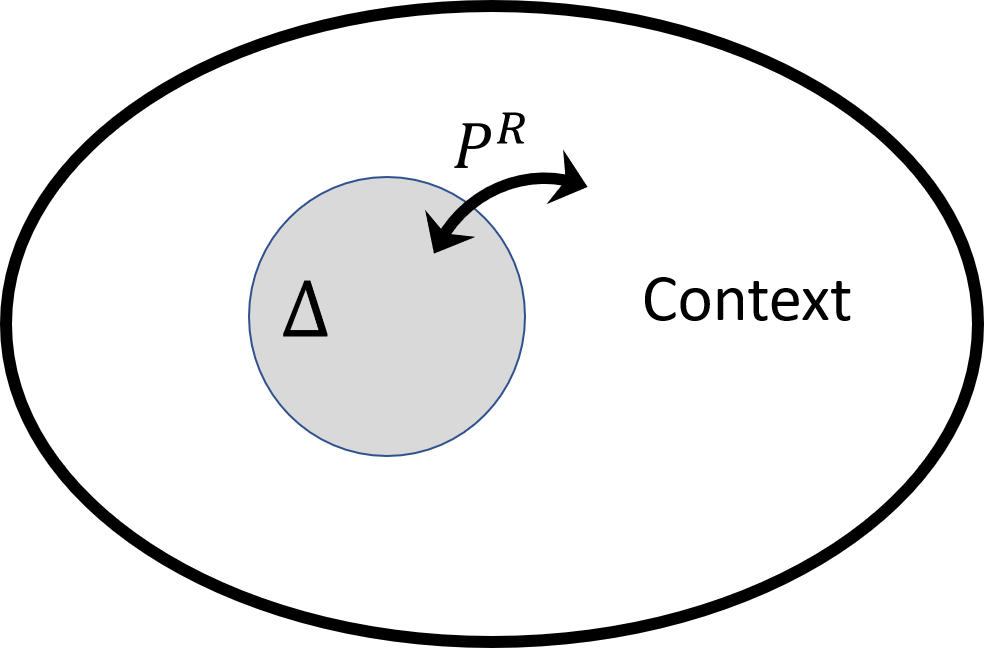
\includegraphics[width= 50mm]{PR.png}
  \caption{Delta-logic}
  \label{pr}
\end{figure}


\paragraph{Advantages of reasoning with Delta-logics:}
Expressing verification conditions in delta-logics has a distinct advantage in automated reasoning. We formulate verification conditions in delta logics in the following manner (see Figure~\ref{blobs}).
We can view the program's transformation of pre-heap to the post-heap as a static model consisting of three different submodels: one is the context heap, the second is the pre-heap restricted to $\Delta$, and the third is the post-heap restricted to  $\Delta$.
Note that there is only one context heap as it does not change, and this context heap is infinite, in general. However, the other two heaps are finite. The recursive properties of the heap are then defined  on the context-heap, parameterized with the communication variables $P_R$ for expressing properties of the pre-heap, and parameterized over the communication variables $P_R'$ for expressing properties of the post-heap.

The key advantage of the above model is that
two of the submodels (both over $\Delta$) are finite, and reasoning about them and the data-fields accessible from them can be automated using standard SMT solvers.
The context heap is the single unbounded submodel that poses automation challenges. In this paper, we exploit this simplicity of dealing only with one infinite submodel (as opposed to the naive formulation, which would have two infinite submodels) to build new powerful classes of decidable logics over lists and list-measures. 

\begin{figure}
  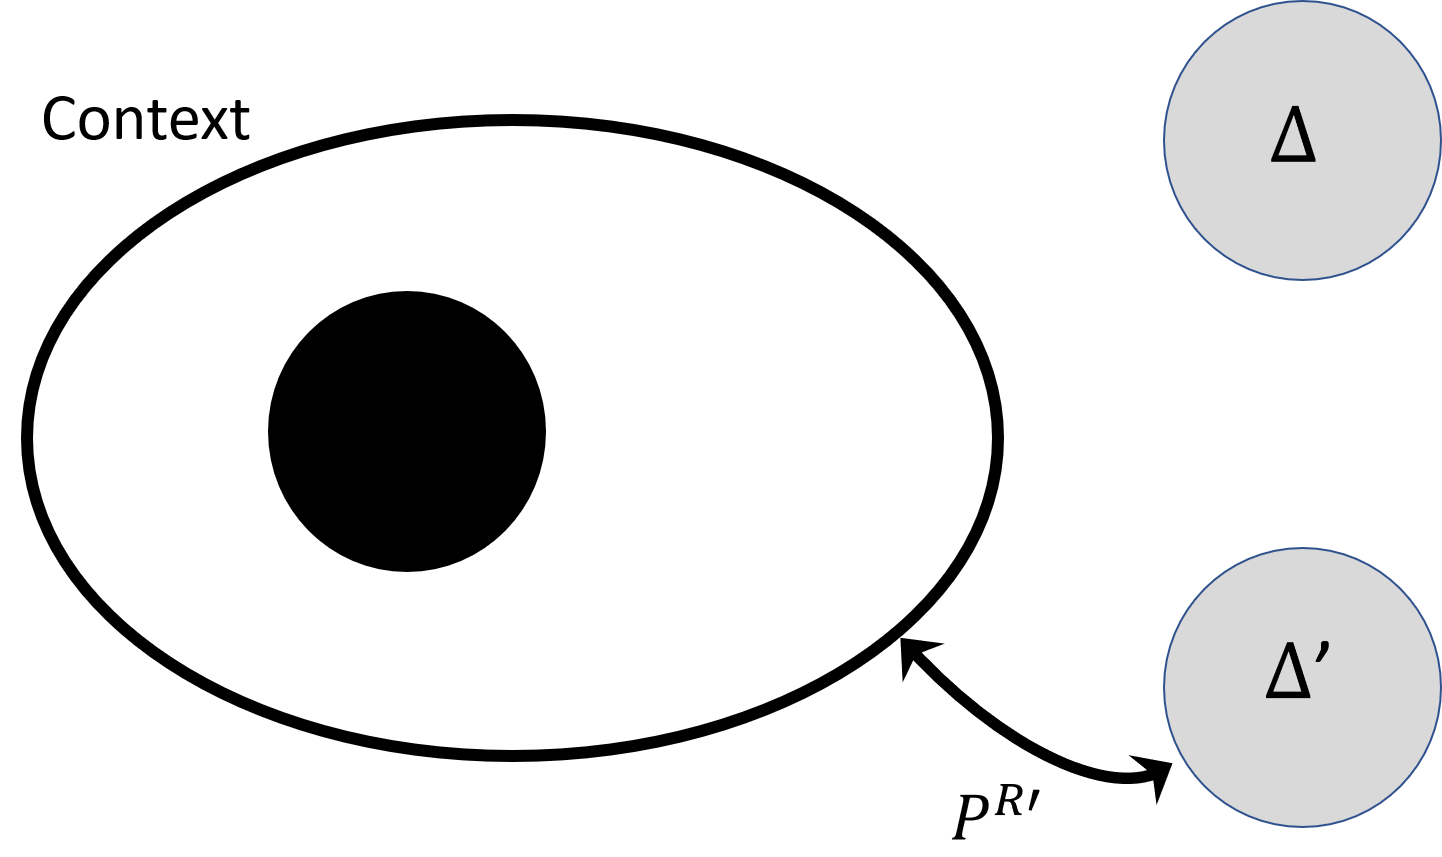
\includegraphics[width= 50mm]{3blobs.png}
  \caption{VC expressed in delta-logics}
  \label{blobs}
\end{figure}


\paragraph{Expressing verification conditions in Delta-logics}
With the above model of verification conditions in mind, let us examine how to write VCs corresponding to Hoare triples in delta-logics. The key idea is to set up parameterized sets of recursive definitions with two sets of parameters $P_R$ and $P_R'$, as described above, expressing the precondition using
one and the postcondition using the other. The program transformation of the $\Delta{}$ portion of the pre-heap to that of the post-heap can be described in quantifier-free FO,  since they are finite.

The main challenge that remains is to express the precondition and postcondition using Delta logics.
%, and the pre- and post-conditions can be translated to delta-logic formulae using the separability theorem. Notice that this captures naturally the changing $\Delta$ portion of the heap while keeping the context unchanged and 
%hence removes the need for the universally quantified formula asserting that pointers in the context have not changed.
In order to do this, we prove a general technical result for delta-logics, called the \emph{separability theorem} in Section~\ref{sec:separability}. This theorem shows that any quantifier-free FO formula
with recursive definitions (with \textit{lfp} semantics) can be expressed in delta-logics: as a boolean combination of delta-specific formulae
and contextual formulae. 

The separation theorem sets up communication between the two portions: the $\Delta$ portion of the heap 
and its context. The context is handled using the parameterized recursive definitions and the $\Delta{}$ portion, being finite, is handled by `unfolding' the recursive definition across $\Delta{}$. This unfolding would stop at the `boundary' of $\Delta{}$ and the context, which is where we use the interface variables to communicate the valuations across these disjoint portions. These are the mutual constraints that were referred to earlier in this section.
However, it turns out that a new set of recursive definitions and communication variables involving a notion of \emph{rank} for each (parameterized) recursive definition is
needed to accurately capture least fixpoints, for the parameterized recursive functions are now merely defined on the context and the \textit{lfp} semantics cannot be preserved by a naive unfolding of the definition, even if the portion on which the unfolding is done is finite (for instance, the familiar definition of lists as either being $nil$ or pointing to a location that points to a list is incorrect with just fixpoint semantics, as it would then be acceptable to call a cycle a list as well). These ranks can, however, be constrained to be \emph{bounded integers} as opposed to ordinals (though the heap is infinite). 


\paragraph{Decidable Delta-logics}
  As a culmination of the above arguments, we demonstrate the efficacy of delta-logics to build a powerful program logic for reasoning with manipulations of lists and list-measures. The decision procedure crucially relies on the simplicity of VCs expressed in delta-logics--- having \emph{one} infinite contextual heap, two finite heaplets and communication between them using only first-order variables.


\subsection{Motivating Example}
\label{sec:motivating_example}
We shall now illustrate our method on a motivating example.
Let us consider the following Hoare triple with pre/post conditions written in FO+\textit{lfp}:\\
\centerline{$ \{ list(x) \wedge  list(w) \wedge  y \not \in hlist(w) \} 
~~~~~\texttt{y.next := w}~~~~~
\{list(x) \}$}\\
where $list(x)$ is a recursive definition that that holds when $x$ points to a list, and in which
case, $hlist(x)$, another recursive definition, captures the set of locations in that list. We omit these definitions.

It is easy to see that this Hoare Triple is valid. First notice that frame reasoning argues that $w$ continues to point to a list.
There are then two cases: if $y$ does not belong to the list pointed to by $x$, then since $y$ is not in the heaplet, frame reasoning would prove that $x$ continues to point to a list.
However, in the case when $y$ does belong to the list pointed to by $x$, we cannot use frame reasoning to immediately conclude that $x$ will continue to point to a list. However, notice that $x$ will point to a list in this case as well, since $y$ will point to $w$ which points to a list. Therefore, frame reasoning \emph{alone} will not be sufficient to conclude the postcondition from the precondition and the program transformation at this point. 

The naive VC for this program is expressed by using a new $next$ pointer (say, $next'$) to model the post-state of the program, redefining the recursive functions and predicates using $next'$ to talk about valuations on the post-state, and observing that $next$ has not changed on any other location except for that pointed to by $y$:

\begin{center}
$\Big( \big( list(x) \wedge  list(w) \wedge  y \not \in hlist(w) \big) \land{} \big( \left(next'(y) = w \land{} y' = y \land{} w' = w \land{} x' = x\right) \land{} \left(\; \forall{}u.\, u\neq{}y \Rightarrow{} next'(u) = next(u)\; \right) \big) \Big) \Rightarrow{} \left(list'(x')\right)$
\end{center}
where the quantifier is interpreted to range over all locations on the heap. We shall now convert this to a VC in delta-logic.

In this case, the set of modified locations is $\Delta{} = \{y\}$. To write the VC in delta-logic we shall first use the separability theorem (Section~\ref{sec:separability}) to write the pre- and and post-conditions in delta-logic. The separability theorem introduces new parameterized \emph{rank} functions for each parameterized recursive definition. For the precondition, this yields a delta-logic formula of the kind:
\begin{center}
 $\left(list^{P}(x) \wedge  list^{P}(w) \wedge  y \not \in hlist^{P}(w)\right) ~~\land{}~~ \beta{}(P)$
\end{center}
where $list^{P}()$ and $hlist^{P}()$ are the parameterized versions with the parameter set $P$. The domain of all of these definitions is the context, and therefore the formula $\left(list^{P}(x) \wedge  list^{P}(w) \wedge  y \not \in hlist^{P}(w)\right)$ is a contextual formula. $\beta{}$ is a delta-logic formula that accurately captures the least fixpoint semantics of the original definitions using the ranks and communication variables $P$. Similarly, we can also write the post-condition in delta-logic as $list'^{Q}(x') \land{} \beta{}(Q)$.

Substituting these into the VC gives:

\begin{center}
$\Big( \big( \left(list^{P}(x) \wedge  list^{P}(w) \wedge  y \not \in hlist^{P}(w) \right) \land{} \beta{}(P) \big) \land{} \big( \left(next'(y) = w \land{} y' = y \land{} w' = w \land{} x' = x\right) \land{} \left(\; \forall{}u.\, u\neq{}y \Rightarrow{} next'(u) = next(u)\; \right) \big) \Big) \Rightarrow{} \left(list'^{Q}(x') \land{} \beta{}(Q) \right)$
\end{center}

We now come to the crux of the versatility of delta-logics in expressing VCs. 
Notice that $list'^Q(x')$ on the
right of the implication above is a \emph{contextual} formula defined using $next'$. However, on the context, $next'$ is precisely $next$. Hence we can replace $list'^Q(x')$ with $list^Q(x')$, the latter being defined in terms of $next$. Since $next'$ is never used on the context, we can drop the universally quantified clause, giving us the VC:

\begin{center}
$\Big( \big( \left(list^{P}(x) \wedge  list^{P}(w) \wedge  y \not \in hlist^{P}(w) \right) \land{} \beta{}(P) \big) \land{} \big( \left(next'(y) = w \land{} y' = y \land{} w' = w \land{} x' = x\right) \big) \Big) \Rightarrow{} \left(list^{Q}(x') \land{} \beta{}(Q) \right)$
\end{center}
It is clear that this is a \emph{quantifier-free} delta-logic formula, and there is only one recursive definition for \emph{list} which is defined using $next$, though it is parameterized with $P$ and $Q$.
\medskip

The problem now reduces to solving for the validity of this VC in delta-logic. In the decidability section (Section~\ref{sec:decidability}), we show exactly how to build an effective procedure to decide the validity of delta-logic formulae over lists with various measures (which, in fact solve this particular example as well; see Section~\ref{sec:experiments}). The problem really is of finding a decision procedure for the solution of contextual formulae. To do this we observe that the context can be abstracted by a finite set of locations, and the list segments between them, if they exist, summarized in a way that can be encoded in SMT. We shall describe this in further detail in Section~\ref{sec:decidability}

\section{Delta Logics}
In this section, we define a general delta-logic extending many-sorted first-order logic with least fixpoints
with background axiomatizations of some of the sorts.

Let us fix a many-sorted first-order signature $\Sigma = (S, {\cal F}, {\cal P}, {\cal C}, {\cal G}, {\cal R})$ where 
$S=\{\sigma_0, \ldots, \sigma_n\}$ is a nonempty finite set of sorts, 
${\cal F}$, ${\cal P}$, and ${\cal C}$ are sets of function symbols, relation symbols,
and constant symbols, respectively, and
${\cal G}$ and ${\cal R}$ are function and relation symbols that will be recursively defined. 
These symbols have implicity defined an appropriate arity and a type signature.


Let $\sigma_0$ be a special sort that we refer to as the \emph{location} sort, which
will model locations of the heap. The other sorts, which we refer to as background sorts, can be arbitrary and
constrained to conform to some theory (such as a theory of arithmetic or a theory of sets).

We assume the following restrictions:
\begin{itemize}
	\item We assume all functions in ${\cal F}$ map either from tuples of one sort to itself or from the foreground
	 sort $\sigma_0$ to a background sort $\sigma_i$. Relations in ${\cal P}$ are over tuples of one sort only.
	\item The functions in ${\cal F}$ whose domain is over the foreground sort $\sigma_0$ are \emph{unary}.
	      Also, relations over the foreground sort $\sigma_0$ are unary relations.
	\item Recursively defined functions (in ${\cal G}$) are all unary functions from the foreground sort $\sigma_0$ 
	         to the foreground sort or a background sort. Recursively defined relations (in ${\cal R}$) are all unary relations on the foreground sort $\sigma_0$.
\end{itemize}

The restriction to have unary functions from the foreground sort (which models locations) is sufficient
to model pointers on the heap (unary functions from $\sigma_0$ to $\sigma_0$) 
and to model data stored in the heap (like the key stored at locations modeled as a function from $\sigma_0$ to a
background sort of integers).
This restriction will greatly simplify the presentation of delta-logics below.
The restriction of having unary recursively defined functions and relations will also simplify the notation.
Note that recursive definitions such as $\textit{lseg}(x,y)$ that are binary can be written recursively
as unary relations such as $\textit{lseg}_y(x)$ (i.e., parameterized over the variable $y$) with recursion
on the variable $x$. 


{\bf Define FO+LFP: syntax and semantics.}




\subsection{Delta Logics}

We parameterize delta logics by a finite set of first-order variables 
$\Delta = \{ v_1, \ldots v_n\}$.

Intuitively, a delta logic formula $\varphi(\vec{x})$ is a formula that evaluates
on a model $M$ while \emph{ignoring} the functions/relations on the locations interpreted
for the variables in $\Delta$. 

More precisely, a semantic definition of the delta logic over $\Sigma$ with respect 
to $\Delta$, is defined as below. First, let us define when a pair of models over the same
universe and an interpretations differ only on $\Delta$.

\begin{definition}[Models differing only on $\Delta$]
Let $M$ and $M'$  be two $\Sigma$-models with universe $U$ that interpret constants the same way,
and let $I$ be an interpretation of variables over $U$.
Then we say $(M, I)$ and $(M', I)$ differ only on $\Delta$ if:
\begin{itemize}
	\item  for every
	function symbol $f$ and for every $l \in U$, $\llbracket f \rrbracket_M(l)  \not = \llbracket f \rrbracket_{M'}(l)$ only if
	there exists some $v \in \Delta$ such that $I(v) = l$.
	
	\item  for every relation symbol $S$ and for every $l \in U$, $\llbracket S \rrbracket_M(l)  \not \equiv \llbracket S \rrbracket_{M'}(l) $ only if 
there exists some $v \in \Delta$ such that $I(v) = l$.\qed	
\end{itemize}
\end{definition}

Intuitively, the above says that the interpretation of the (unary) functions and relations of the two models are 
precisely the same for all elements in the universe that are not interpretations of the variables in $\Delta$.

An FOL+lfp formula over $\Sigma$, $\varphi(\vec{x})$, is a delta-logic formula
if the formula does not distinguish between models that differ only on $\Delta$:


\begin{definition}[Delta-logic formulas]
An FOL+lfp formula over $\Sigma$, $\varphi(\vec{x})$, is a delta-logic formula
if for every two $\Sigma$-models $M$ and $M'$ with the same universe and every interpretation $I$ 
such that $(M, I)$ and $(M', I)$ differ only on $\Delta$, 
$M, I \models \varphi$ iff $M', I \models \varphi'$.\qed
\end{definition}

Delta-logic formulae can be easily written using syntactic restrictions where the formula (and the recursive definitions)
are written so that every occurrence of $f(t)$ (where $f$ is a function symbol) or $P(t)$ (where $P$ is a relation symbol),
where $t$ is a term of type $\sigma_0$, 
is guarded by the clause ``$t \not \in \Delta$'', which is short for $\bigwedge_{v \in \Delta} t \not = v)$.

\noindent Let us now give some examples of delta-logic formulae.

\paragraph{Example:}
\emph{
Let us fix a finite set $\Delta$ of first-order variables.\\
The recursive definition $$\textit{ls}(x) :=_{\textit{lfp}} (x=\textit{nil} \vee (x \not = nil \wedge x \not \in \Delta \wedge \textit{ls}(n(x))) 
 \vee (x \not = nil \wedge \bigvee_{v \in \Delta} (x\!=\!v \wedge b_v)))$$ 
 is a delta-logic definition with respect to $\Delta$.
The above defines lists where by ``imbibing'' facts about whether a location $v$ in $\Delta$ is a list using the
free Boolean variable $b_v$. The definition says that $x$ points to a list if it either is equal to the constant $\textit{nil}$,
or is not equal to $\textit{nil}$ and either $x$ is not in $\Delta$ and $n(x)$ is a list or $x$ is in $\Delta$, and the corresponding
Boolean variable holds. The least fixpoing semantics of the above definition gives a unique definition: $ls(u)$ is true iff
there is a path using the pointer $n()$ that either ends in $\textit{nil}$ or ends in a node $v$ in $\Delta$ where $b_v$ is true. 
Note that the formula $n(x)$ is guarded by the check $x \in \Delta$, and hence this is a delta-logic formula.
Changing the model to reinterpret $n()$ over $\Delta$ (but preserving the interpretation of the variables $b_v$, $v \in \Delta$) 
will not change the definition of $\textit{ls}$ in any way.
}

\emph{The formula $u \not \in \Delta \wedge u'\!\!=\!\!n(u) \wedge \textit{ls}(u')$ is a delta-logic formula that uses the above definition
	(note that the formula $n(u)$ is again guarded by a check ensuring $u$ is not in $\Delta$). Again, changing the interpretation 
	 of $n()$ on $\Delta$ will not affect the truth of this formula (provided the interpretation of $u$ and $u'$ do not change).
}


\section{Translating Verification Conditions to Delta Logics}


\section{A Decidable Delta Logic on Lists with List Measures}

In this section, we will define a delta logic on linked lists equipped with \emph{list measures}--- measures of
list segments that include length, its heaplet, the multiset of keys stored in the list (say, in a data-field {\tt key}),
and the minimum and maximum keys stored in it. We prove that the quantifier-free first-order logic fragment of this delta logic 
is \emph{decidable}. More precisely, we show that the logic can be translated to an equisatisfiable quantifier-free first-order
formula that is decidable by using a Nelson-Oppen combination of decidable theories of arithmetic, sets, and uninterpreted functions.
The translation in fact will allow us to decide formulas of the form $\alpha \wedge \beta$ obtained as verification conditions
in the section above, where $\alpha$ is a delta-logic formula on lists and list measures and $\beta$ is over a decidable
Nelson-Oppen combinable quantifier-free theories, and where $\alpha$ and $\beta$ share Boolean and first-order variables.
At the end of the section, we outline some generalizations of our result.

\subsection*{A delta logic over list measures}
As usual, let us fix a set of first-order variables $\Delta$.
Let us also fix a single pointer field $n$.

\begin{definition}[Recursive Definitions for the Logic of List Measures (LM)]
Let us fix a set of \emph{parameter variables} $P$ that consists of a tuple of sets of variables:
a set of Boolean variables $LS_z^v$, a set of variables with type set of locations
$HLS_z^v$, a set of variables of type multiset of keys $MSKEYS_z^v$, and
a set of variables of type integer $Max_z^v$ and $Min_z^v$, where $z,v$ range over $\Delta$.

The delta-logic of list measures (LM) wrt $\Delta$ and parameter variables $P$ is defined using the following recursive definitions, which depend crucially on the parameter variables $P$.
\begin{itemize}
	\item We have unary relations $ls_z^P$ that capture linked list segments 
	       that end in $z$, where
	         the relation for a location $v$ in $\Delta$ is imbibed using the Boolean variables $LS_z^v$ ($v \in \Delta$),
	      and where $z$ is any element of $\Delta$ or the constant location $\textit{nil}$.
	      (The relation $ls_\textit{nil}()$ captures whether a location points to a list
	       ending with $\textit{nil}$.)
	
	This is defined as follows:
	$$\textit{ls}_z^P(x)\!\!:=_{\textit{lfp}}\!\! \left( x\!\!=\!\!\textit{z} \vee \left( x \!\not =\! z \wedge x \!\not=\! nil \wedge x \not \in \Delta \wedge \textit{ls}_z^P(n(x))\right) 
	\vee\right.$$
	$$~~~~ \left.\left(x \!\not =\! z \wedge x \in \Delta \wedge \bigwedge_{v \in \Delta} (x=v \Rightarrow LS_z^v)\right)\right)$$ 
	           

    \item We have recursive definitions that capture the heaplet of such list-segments, where the heaplet
of list-segments from an element $v$ in $\Delta$ to $z$ (where $z \in \Delta \cup \{nil\}$) is imbibed from the set variable $\HLS_z^v$:
\begin{align*}
\textit{hls}_z^P(x) & :=_{\textit{lfp}} & \emptyset & \textit{~~if~} \sem{x}\!\!=\!\!\sem{z} \\
& & \{x\} \cup \textit{hls}_z^P(n(x)) & \textit{~~if~} \sem{x} \!\not =\! \sem{z} \wedge \sem{x} \!\not=\! \sem{nil} \wedge \sem{x} \not \in \sem{\Delta} \\
& & \HLS\,_z^v & \textit{~~if~} \sem{x} \not = \sem{z} \wedge \sem{x}=\sem{v} \wedge v \in \Delta 
\end{align*}

    \item We have recursive definitions that capture the multiset of data elements (through a data-field
    $\textit{key}$) stored in list segments, 
    where again the multiset of data 
of list-segments from an element $v$ in $\Delta$ to $z$ (where $z \in \Delta \cup \{nil\}$) is imbibed from the set variable $MSKeys_z^v$:
\begin{align*}
\textit{mskeys}_z^P(x) & :=_{\textit{lfp}} & \emptyset & \textit{~~if~} \ \sem{x}\!\!=\!\!\sem{z} \\
& & \{\textit{key}(x)\} \cup_m \textit{mskeys}_z^P(n(x)) & \textit{~~if~} \sem{x} \!\not =\! \sem{z} \wedge \sem{x} \!\not =\! \sem{nil} \wedge \sem{x} \not \in \sem{\Delta} \\
& & \textit{MSKeys}_z^x & \textit{~~if~} \sem{x} \!\not =\! \sem{z} \wedge \sem{x}=\sem{v} \wedge v \in \Delta 
\end{align*}

    \item We have recursive definitions that capture the maximum/minimum element of data elements stored in list segments, where again the maximum/minimum element  
of list-segments from an element $v$ in $\Delta$ to $z$ where $z \in \Delta \cup \{nil\}$) is imbibed from the data variable $Max_z^v$ (or $Min_z^v$).
We assume the data-domain has a linear-order $\leq$, and that there are special constants $-\infty$ and $+\infty$
that are the minimum and maximum elements of this order. Let $max(r_1,r_2) \equiv \textit{ite}(r_1 \leq r_2, r_2, r_1)$.
\begin{align*}
\textit{Max}_z^P(x) & :=_{\textit{lfp}} & -\infty & \textit{~~if~} \sem{x}\!\!=\!\!\sem{z} \\
& & \textit{max}(key(x), \textit{Max}_z^P(n(x))) & \textit{~~if~} \sem{x} \!\not =\! \sem{z} \wedge \sem{x} \!\not=\! \sem{nil} \wedge \sem{x} \not \in \sem{\Delta} \\
& & \textit{MSKeys}_z^v & \textit{~~if~} \sem{x} \not = \sem{z} \wedge \sem{x} = \sem{v} \wedge v \in \Delta 
\end{align*}

 The function $\textit{Min}_z^P$ is similarly defined.
 
    \item We have a recursive definition that captures sortedness, using the minimum measure.
\begin{align*}
	&\textit{Sorted}_z^P(x) \!\!:=_{\textit{lfp}}\!\! \Big( ~~x\!\!=\!\textit{z} ~~\vee  \\
	&~\left( x \!\not =\! z \wedge x \!\not=\! nil \wedge x \not \in \Delta \wedge \textit{min}_z^P(x) \!\not =\! \bot \wedge \textit{key}(x) \leq \textit{min}_z^P(x) \wedge \textit{Sorted}_z^P(n(x))\right) \vee\\
&	~
\left(x \!\not =\! z \wedge x \in \Delta \wedge \textit{min}_z^P(x) \!\not =\! \bot \wedge \textit{key}(x) \leq \textit{min}_z^P(x) \wedge \bigwedge_{v \in \Delta} (x=v \Rightarrow \textit{SORTED}_z^v\right)\Big)
\end{align*}

\end{itemize}
\end{definition}

The above definitions can be written in usual syntax using $\textit{ite}$ expressions; we omit this 
formulation.

We define the \emph{context logic of list-measures (LM)} to be quantifier-free formulas that use only the recursive 
definitions of $LM$ mentioned above, and combine them as described in Figure~1.
The logic $LM$ allows first-order variables that range over locations, keys, and integers. Note that
dereferencing pointers of locations is completely disallowed--- the delta-specific formula that combined
with context logic formulas will refer to such dereferences, depending on the particular state modeled.
Here $\Delta$ is assumed to be a subset of the free location variables in the context logic formula.


$LM$ formulas are ; the subformulae of the formula in $LM$ are however allowed
to refer to \emph{different} sets of parameter variables.

\begin{figure}
   \begin{align*}
   \textit{Location} ~~\textit{Term} ~~lt & ::=  x \mid p_i(y) \mid \texttt{nil} \hfill*{\textit{~~~~~~~~~~~~~where~} y \not \in \Delta}\\
   \textit{Integer} ~~\textit{Term} ~~it & ::=  c \mid len_z^P(lt) \mid it+it \\
   \textit{Key} ~~\textit{Term} ~~keyt & ::=  c \mid \textit{key}(lt) \mid max_z^P(lt) \mid min_z^P(lt) \mid keyt+keyt \\
   \textit{Heaplet}~~ \textit{Term} ~~hlt  & ::=  \emptyset \mid \{ lt \} \mid hls_z^P(lt) \mid hlt \cup hlt \mid hlt \cap hlt \mid hlt \setminus hlt\\
   \textit{MultisetKeys}~~ \textit{Term} ~~mskt & ::= \emptyset \mid mskeys_z^P(x) \mid mskt \cup_m mskt \mid mskt \cap_m mskt \mid mskt \setminus_m mskt\\
   ~&~\\
   \textit{Formulas}~~ \varphi &  ::=  b \mid ls_z^P(x) \mid sorted_z^P(x) \mid lt = lt \mid lt \in hlt \mid hlt \subseteq hlt \mid hlt = \emptyset \mid \\
   ~& ~~~~~ it < it \mid it = it \mid keyt < keyt \mid keyt = keyt \mid \\
   ~& ~~~~~ keyt \in mskt \mid mskt \subseteq_m mskt \mid \varphi \vee \varphi \mid \neg \varphi
   \end{align*}
 \caption{The context logic $LM$ of list measures involving list-segments, heaplets, multisets of keys, max, min, and sortedness.} 
\end{figure}



\subsection{Deciding the logic of list measures}
We can now state the main result of this section:

\begin{theorem}
	Given a quantifier-free formula $\varphi(\vec{x})$ in LM with recursive definitions
	of $ls$ and measures of length, heaplet, keys, max, and min, there is
	an effective procedure that constructs a quantifier-free FOL formula $\psi(\vec{x})$ over 
	a decidable Nelson-Oppen combination of theories of quantifier-free Presburger arithmetic, 
	sets with cardinality constraints, and uninterpreted functions such that for \emph{any}
	interpretation of the variables $\vec{x}$, there is a model that satisfies $\varphi$ iff there
	is a model that satisfies $\psi$.
\end{theorem}


\begin{corollary}
	 The satisfiability problem for quantifier-free $LM$ formulas is decidable.
\end{corollary}

Let us fix a set of sets of parameters ${\cal P} = \{P_1, \ldots P_k\}$
(we encourage the reader to fix $k=2$ in their mind while reading the section, as it's the
most common and the logic VCs translate to, as shown in Section~\ref{}).

We will first describe the decision procedure and its proof of correctness for the fragment
of $LM$ that involves only the three recursive definitions $ls_z^P$, $hls_z^P$, and $rank_z^P$,
where $P \in \{\cal P\}$, which we will refer to as $LM[ls,hls,rank]$. 
Then we will extend the procedure to handle the logic with all the other measures; this latter
proof requires more expressive decision procedures and pseudo-measures that make its proof harder.

Let us assume a quantifier-free $LM[ls,hls,rank]$ formula $\varphi$ which is a $\Delta$-logic formula
wrt a finite set of variables $\Delta$.
Assume the (free) location variables occurring in $\varphi$ is $X = \{x_1, \ldots x_n\}$ with
$\Delta \subseteq X$. 

In order to determine whether there is a model satsifying $\varphi$, we need to construct a universe
of locations, an interpretation of the variables in $X$, and the heap
(with the single pointer field $n()$) on all locations \emph{outside} $\Delta$ (the definition
of $n()$ on $\Delta$, by definition, does not matter).

Our decision procedure intuitively relies on the following observations. First, note that the locations
reached by using the $n()$ pointer any number of times forms the relevant set of locations that $\varphi$'s
truth can depend on (as $\varphi$ is quantifier-free and has recursive definitions that only use the $n$-pointer).
When pursuing the paths using the $n$-pointer on a location $x$, there are three distinct cases that can happen:
(a) the path may reach a node in $\Delta$, (b) the path may reach a node that is reachable also from another location in $X$,
or (c) the path may never reach a location in $\Delta$ nor a location that is reachable from another location in $X$. 

The key idea is to \emph{collapse} paths where the reachability of them from variables in $X$ does not change.
More precisely, let $L$ be the set of all locations reachable from $X$ such that $l$ is in $\Delta$ or 
for every location $l'$ reachable from $X$ such that $n(l')=l$, the set of nodes in $X$ that have a path
to $l'$ is different from the set of nodes in $X$ that have a path to $l$.

It is easy to see that there are at most $|X|-1$ locations of the above kind that are distinct from $\Delta$,
since the paths can merge at most $|X|-1$ times forming a tree-like structure. Our key idea is now to 
represent these list segments that connect these kinds of locations \emph{symbolically}, summarizing the 
measures on these list segments. Since there are only a bounded number of such locations and hence list
segments, we can compute recursive definitions of linear measures involving them using quantifier-free
and recursive-definition-free formulae.

We construct a formula $\psi$ that is satisfiable iff $\varphi$ is satisfiable, as follows.
First, we fix a new set (distinct from $X$) of location variables $V={v_1, \ldots v_{|X|-1}}$,
to stand for the merging locations described above.
We introduce an uninterpreted function $T: V \cup (X\setminus \Delta) \longrightarrow V \cup X \cup \{\bot\}$.
Let $Z$ be the set of variables in $\Delta$ as well as the variables in $X \setminus \Delta$ 
such that the recursive definitions $ls_z^P$, $hls_z^P$, $rank_z^P$, for some
$P \in {\cal P}$, occurs in $\varphi$.

\medskip
\noindent 
{\bf $\psi$ is the conjunct of the following formulas:}
\begin{itemize}
	\item The formula $\varphi$ (but with recursive definitions treated as uninterpreted relations and functions).
	\item For every $z \in Z$, we introduce an uninterpreted function $Dist_z: V \cup (X \setminus \Delta) \longrightarrow \mathbb{N} \cup \{\bot\}$ that
             is meant to capture the distance from any location in $V \cup X$ to $z$, if $z$ is reachable from
               that location without going through $\Delta$, and is $\bot$ otherwise. We add the constraint:
          $$\bigwedge_{v \in V\cup (X\setminus \Delta)} \big[ (Dist_z(v)\!=\!0 \Leftrightarrow v=z) ~\wedge ~~~~~~~~~~~~~~~~~~~~~~~~~~~~~~~~~~~~~~~~~~~~~~~~~~~~~~$$
          $$ v \!\not =\! z \Rightarrow \big(~\left( (T(v)\!=\!\bot \vee Dist_z(T(v))\!=\!\bot) \Rightarrow Dist_z(v) \!=\! \bot
                 \right)~~~~~~~~~~~~~~~$$
          $$  ~~~~~  \left. \wedge ~((T(v) \not = \bot \wedge Dist_z(T(v)) \not = \bot) \Rightarrow Dist_z(v) = Dist_z(T(v))+1
                \big) ~\right)\big] $$
              
	\item For every $x \in X$, and for every $P \in {\cal P}$, we have a conjunct:
		     $$ls_z^P(x) \Leftrightarrow (Dist_z(x)\not= \bot \vee \bigvee_{v \in \Delta} (Dist_v(x) \not = \bot
		       \wedge LS_z^v))$$
		     
    \item For every $x \in X$, $z \in Z$, and for every $P \in {\cal P}$, we have a conjunct:
             $$ \left( Dist_z(x) \!=\! \bot \Rightarrow rank_z^P\!(x)\!=\!\bot\right) ~~\wedge~~ 
               \left( Dist_z(x) \!\not =\! \bot \Rightarrow rank_z^P\!(x)\!=\!RANK_z^P \right)$$
               
    \item We capture the heaplets of list-segments from $v \in V \cup (X \setminus \Delta)$ to $T(v)$ (excluding both
              end-points) using a set
             of locations $H(v)$
             and constrain them so that they are pairwise disjoint and do not contain the locations $X$:
             $$ \bigwedge_{x \in X, v \in V \cup (X \setminus \Delta)} x \not \in H(v) ~~\wedge 
             \bigwedge_{v,v' \in V \cup (X \setminus \Delta)} (v \!\not =\! v' \Rightarrow H(v) \cap H(v') = \emptyset)$$  
    
    \item We can then precisely capture the heaplet $hls_z^P(x)$ by taking the union of all heaplets of
           list segments lying on its path to $z$. We do this using the following constraint, for each
           $v \in X \cup V$:
           $$(Dist_z(v)=\bot \Rightarrow hls_z^P (v) = \emptyset) \wedge (hls_z^P(z)= \emptyset)\wedge $$
           $$(Dist_z(v) \not = \bot \wedge v \not = z) \Rightarrow hls_z(v)= H(v) \cup \{v\} \cup hls_z(T(v))$$

\end{itemize}

Note that the formula $\psi$ is quantifier-free and over the combined theory of arithmetic, uninterpreted functions, and sets.

We can show the correctness of the above translation:
\begin{theorem}
	For any quantifier-free formula $\varphi({\cal P}, X)$ of $LM[ls,hls,rank]$, the quantifier-free and recursion-free
	 formula $\psi({\cal P}, X)$ obtained $\varphi$ obtained from the translation above
	 satisfies the following property: for any interpretation of the free variables
    in ${\cal P} \cup X$, there is a model for $\varphi$ iff there is a model for $\psi$.
\end{theorem}

\bigskip

We now turn to the more complex logic $LM[ls, hls, rank, len, mskeys, min, $\\$max, sorted]$, and show that
any quantifier-free formula $\varphi$ in the logic can be satisfied. First, we model the multi-set
of keys, minimum and maximum values and sortedness of each list-segment from $v$ to $T(v)$ 
(where $v \in (X \setminus \Delta) \cup V$),
which is outside $\Delta$, using multiset variables $mskeys\mu(v)$, integer variables $min\mu(v)$, $max\mu(v)$,
and $len\mu(v)$ and Boolean variables $sorted\mu(v)$.
We can also aggregate them, as above, to express the sets $mskeys_z(x)$, $min_z(x)$, $max_z(x)$, $len_z(x)$
and $sorted_z(x)$, for each $z \in Z$ and
each $x \in (X \setminus \Delta) \cup V$, similar to definitions of $hls_z(x)$ as defined above.
One point to note is that the recursive definition of sortedness across segments will by expressed
by using both $Min_z(x)$ and $Max_z(x)$ definitions, though the definition of sortedness is defined
using only minimum--- this is needed as expressing when concatenation of sorted list segments is sorted
requires the max value of the first segment. We skip these definitions as they are easy to derive.

The main problem that remains is in \emph{constraining} these measures so that they can be the measures
of the \emph{same} list segment. The following constraints capture these constraints, for each 
$v \in (X \setminus \Delta) \cup V$:
\begin{itemize}
	\item The cardinality of $hls\mu(v)$ must be $len\mu(v)$.
	\item The cardinality of $mskeys\mu(v)$ must be $len\mu(v)$.
	\item $min\mu(v)$ and $max\mu(v)$ must be the minimum and maximum elements of $mskeys\mu(v)$.
	\item If $min\mu(v)=max\mu(v)$ (and they are not $\bot$), then $sorted\mu(v)$ can only be true.
\end{itemize}

The intuition is that any measures meeting the above constraints can be realized using true list
segments. As for the third clause above, notice that any list segment with minumum element different
from maximum can be realized using either a sorted list or an unsorted list.

The above constraints on measures, though seemingly simple, are hard to shoehorn into existing decidable theories
(though the third constraint can be easily expressed).
The first constraint can be expressed using quantifier-free BAPA~\cite{} (Boolean Algebra with Presburger
arithmetic) constraints, which is decidable. We can get around defining the minimum of list segments
by having the set of keys store only offsets from the minimum (and including the key $0$ always). However,
capturing max and sortedness measures in addition while preserving decidability seems hard.

Consequently, we give a new decision procedure that exploits the setup we have here.
First, note that we can restrict the formulas that use the keys stored in sets to involve
only membership testing of free variables in them, combinations using union and intersection,
and checking emptiness of derived sets. We can \emph{disallow checking non-emptiness} as non-emptiness
of a set $S$ can always be captured by demanding $k \in S$, for a freshly introduced free variable $k$
without affecting satisfiability.

Our primary observation is that we can then restrict the multiset of keys to be over a  \emph{bounded}
universe of elements. This bounded universe will consist of one element for each free variable of type key 
in the formula (call this $K$), and in addition will consist of one element for each Venn region formed by the multiset
of keys for each segment $(v,T(v))$ of the context heap. The idea of introducing an element for each Venn
region is not new, and is found in many works that deal with combinations of sets and cardinality constraints~\cite{}.

One can show that if there is a satisfiable model, then by collapsing all elements that are different
than $K$ and that are in the same Venn region can be identified by the unique representative we have chosen
for that region. Taking unions and intersections will not affect the multiplicities of elements in the Venn
region and the formula cannot distinguish between them (as it is quantifier-free).

Once we have bounded the universe of keys, we can represent a multiset of keys using a set of natural numbers
that represent the multiplicity of elements in the multiset, and write the effect of unions and intersections
using Presburger arithmetic. The cardinality of the multiset can be expressed as the sum of these numbers
and the minimum and maximum key can be expressed using the smallest and largest keys in the finite universe
with multiplicity greater than $0$. 
We can hence translate the formula into a quantifier-free formula, 
giving the required theorem.

Note that the above procedure introduces an exponential number of variables, and hence poses challenges
to be effective in practice. There are several possible ways we see to mitigate it. 
First, there is existing work~(see ~\cite{}) on reasoning with BAPA that argues and builds practical 
algorithms that introduce far smaller universes in practice. Second, in the case where we allow only
combinations of sets using union (and not intersection), and allow checking subset constraints and emptiness,
we can show that introducing a \emph{single} new element in the universe other than $K$ suffices. The reason
is that when there are no intersections, the identity of the elements do not matter and their multiplicities
are preserved by representing with only one element. It turns out that there are many instances in verification
of programs where the intersection of multisets of keys is never called for (intersection of \emph{heaplets} are
very important as they are needed to model separation, but we handle them using true sets as described earlier).
Third, as we explain in the evaluation section, we can use some approximations of the constraints to obtain
faster procedures, and this already seems to work adequately in practice.

We end with the main theorem:
\begin{theorem}
	For any quantifier-free formula $\varphi({\cal P}, X)$ of $LM[ls, hls, rank, len, $\\$min, max, sorted]$, the quantifier-free and recursion-free
	formula $\psi({\cal P}, X)$ obtained $\varphi$ obtained from the translation above
	satisfies the following property: for any interpretation of the free variables
	in ${\cal P} \cup X$, there is a model for $\varphi$ iff there is a model for $\psi$.
\end{theorem}


	\section{Separability Theorem}
In this section, we show a key result: that for any quantifier-free FO+\textit{lfp} formula we can effectively find an equivalent delta-logic formula. We do this by reasoning separately with the elements of the formula that are specific to $\Delta{}$, and those that are oblivious to $\Delta{}$. We bring these separate analyses together with a set of parameters that we shall describe and justify below.\\\

First, let us consider a recursively defined function $R$, with the restricted in form as above \ref{make sure those restrictions are written}. Let the set of functions $PF = \{ p_i \,|\, 1 \leq{} i \leq{} k \}$ (for some $k$) model the pointer fields (we assume that have a clause $p_i(nil) = nil$ for every $1 \leq{} i \leq{} k$). We also assume that $\Delta{}$ is fixed for this discussion.\\
We define a set of variables $\{R^{d}\,|\, d \in{} \Delta{} \}$ of the type of the range of $R$. These variables are in the set of parameters $P$. Then if $R$ is defined as $R(x) :=_\textit{lfp} \varphi{}(x)$ we define a new function corresponding to $R$, namely $R^{P}$, that is recursively defined as follows:\\
\begin{align}
R^{P}(x) & :=_\textit{lfp} & R^{d} & \textit{ if } \llbracket{}x\rrbracket{} = \llbracket{} d \rrbracket{} \textrm{ for some } d \in{}\Delta{}\tag{delta case}\\
& & \varphi{}[R^{P}/R] & \textit{ if } \llbracket{}x\rrbracket{} \notin{} \llbracket{}\Delta{}\rrbracket{} \tag{recursive case}
\end{align}  
It is easy to see that for a formula $R(x)$, writing it as $R^{P}(x)$ would be a formula in context-logic since any model of it would not depend on a valuation of $PF$ over $\Delta{}$.\\\

To capture the semantics of the original \textit{lfp} definition, we constrain these parameters. This will yield definitions that are equivalent in FO+\textit{lfp} under such constraints.\\
We do this by writing constraints that, effectively, unfold the recursive definition over $\Delta{}$. However in doing so we would run into a problem with cycles. Consider the case of evaluating a list predicate at a node by simply imbibing the value from the node pointed to when we have a circular list.\\
We handle this by introducing the notion of the `rank' of a location w.r.t $R$. In particular, for the example of a circular list, if we recursively defined rank as a natural number increasing on a list starting from $0$ at the location $nil$, there is no way to provide a valuation of every element on the cycle as pointing to a list. However, since the rank will need to communicate through the elements outside $\Delta{}$ to maintain this order (pointer paths between elements interpreted in $\Delta{}$ need not lie within it), it will also be a similarly relativised \textit{lfp} definition with a set of parameters $\{\textit{RANK}_{R}^{d} \,|\, d \in{} \Delta{} \}$ which are also included in $P$. We choose to model the rank as a function to $\mathbb{N} \cup{} \{\ bot{}\}$ ($\bot{}$ signifies undefined rank) as follows given recursively defined function $R$:

\begin{align*}
Rank_{R}(x) & :=_\textit{lfp} & \textit{RANK}_{R}^{d} & \textit{ if } \llbracket{}x\rrbracket{} = \llbracket{}d\rrbracket{} \textrm{ for some } d \in{}\Delta{} \tag{delta case}\\
& & 0 & \textit{ if } \llbracket{}x\rrbracket{} \notin{} \llbracket{}\Delta{}\rrbracket{} \land{} R^{P}(x) \neq{} \bot{} \land{}\bigvee\limits_{1 \leq{} i \leq{} k}\left( R^{P}(p_i(x)) = \bot{}\right) \tag{base case}\\
& & \max\limits_{1 \leq{} i \leq{} k}\{Rank_{R}(p_i(x))\} & \textit{ if } \llbracket{}x\rrbracket{} \notin{} \llbracket{}\Delta{}\rrbracket{} \land{} R^{P}(x) \neq{} \bot{} \tag{recursive case}\\
& & \bot{} & \textit{ if } \llbracket{}x\rrbracket{} \notin{} \llbracket{}\Delta{}\rrbracket{} \land{} R^{P}(x) = \bot{}\tag{undefined}
\end{align*}

Finally, we define some more parameters in $P$ in similar vein as above to communicate between the constraints within $\Delta{}$ and the new \textit{lfp} definitions that are in context-logic. This will be on variables in $p_i(\Delta{}) \cap{} \Delta^{c}$ for some $i$, and are therefore named thus:\\
Let $R^{p_i(\Delta)} = \{ R^{p_i(d)} \,|\, d \in{} \Delta{} \}$ of the type of range of $R$\\
and $\textit{RANK}_{R}^{p_i(\Delta)} = \{ \textit{RANK}_{R}^{p_i(d)} \,|\, d \in{} \Delta{} \} \subseteq{} \mathbb{N} \cup{} \{\bot{}\}$\\
for every $1\leq{} i \leq{}k$.\\\

We then denote the substitution $\varphi(x)[P_{R}/R]$ as replacing the term $R(p_i(x))$ with $R^{p_i(x)}$ for every $1\leq{} i \leq{}k$, and $\varphi(x)[\bot{}/R]$ as replacing with $\bot{}$.
With the above, we write the following delta-specific constraint $\beta_{R}$ for a recursively defined function $R$:\\

\begin{align*}
\bigwedge\limits_{d \in{} \Delta} \big\lbrack{} & \left( \varphi{}(d)[\bot{}/R] \neq{} \bot{} \implies{} R^{d} = \varphi{}(d)[\bot{}/R] \land{} \left(\textit{RANK}_{R}^{d} = 0\right) \right)\tag{base case}\\
&\land{}  \left( \left( \varphi{}(d)[\bot{}/R] = \bot{} \land{} \varphi{}(d)[P_{R}/R] \neq{} \bot{}  \right) \implies{} \left( R^{d} = \varphi{}(d)[P_{R}/R] \right.\right.\notag{}\\
&\qquad{} \left.\left. \land{} \left(\textit{RANK}_{R}^{d} = \max\limits_{1 \leq{} i \leq{} k}(\{\textit{RANK}_{R}^{p_i(d)} \}) + 1 \right)\right)  \right) \tag{recursive case}\\
& \land{}  \left( \left( \phi{}(d)[\bot{}/R] = \bot{} \land{} \phi{}(d)[P_{R}/R] = \bot{} \right) \implies{} \left( R^{d} = \bot{} \land{} \left(\textit{RANK}_{R}^{d} = \bot{} \right)\right) \right) \big\rbrack{} \tag{undefined}
\end{align*}\\

The above constraints capture the values of $R$ accurately on $\Delta{}$:
\begin{itemize}
\item{} the base case simply constrains the parameter at a node interpreting its corresponding variable to be the value provided by the function definition, and its rank to be $0$ when the interpretation for that variables satisfies the base case of the recursive definition.

\item{} the recursive case constrains the parameter (when it does not satisfy the base case) to be the value computed by one unfolding of the definition, where the values of the descendants are also denoted by their respective parameters (whether $\Delta{}$ or boundary) and its rank to be one more than the maximum rank among its descendants.

\item{} the undefined case constrains the parameter to be undefined when it must be according to an unfolding of the definition, and its rank to be undefined as well.
\end{itemize}

Lastly, we must also have that the `boundary' does in fact communicate the values of the context-logic recursive definition to $\Delta{}$, i.e that the placeholder parameters for their values are indeed the values provided by the context-logic \textit{lfp} definition:\\ 
\begin{align*}
\bigwedge\limits_{1 \leq{} i \leq{} k} \big\lbrack{} p_i(d) \notin{} \Delta{} \implies{} & \left( R^{p_i(d)} =  R^{P}(p_i(d)) \right) \notag{}\\
& \land{} \left( \textit{RANK}_{R}^{p_i(d)} =  Rank_{R}(p_i(d)) \right) \big\rbrack{} \notag{} 
\end{align*}
These constraints ensure that the values of the function are computed accurately on $\Delta{}$.\\\

We are now ready to state the main theorem, the proof of which will use the following lemma. Let $P$, which we shall write as $P_{R}$ to indicate the function, include only the sets of parameters defined hitherto. Then: 

\begin{lemma}
\label{relative_lfp}
For any recursively defined function $R$, $\left(\exists{}P_{R}.\,\,\beta_{R} \right) \land{} \left(\forall{}P_{R}.\,\left(\beta_{R} \implies{} R^{P_{R}} = R\right) \right)$
\end{lemma}

If this is true then we have for any FO+\textit{lfp} formula $\alpha$ an equivalent delta-logic formula. Let the set of recursive functions/predicates mentioned in $\alpha{}$ be $\mathcal{R}$, and $\Delta{}$ be fixed. Let $\mathcal{R}^{P} = \{ R^{P_{R}} \,|\, R \in{} \mathcal{R}\}$, and $P_{\mathcal{R}} = \bigcup\limits_{R \in{} \mathcal{R}}P_{R}$. Then:\\

\begin{theorem}[Separability]
$\alpha{} \equiv{} \exists{}P_{\mathcal{R}}.\, \alpha[\mathcal{R}^{P}/\mathcal{R}] \land{} \left( \bigwedge\limits_{R \in{} \mathcal{R}} \beta_{R} \right)$.
\end{theorem}

\begin{proof}
Consider that $\alpha{}$ holds. From lemma \ref{relative_lfp}, for every $R \in{} \mathcal{R}$, we can pick $P_{R}$ such that $\beta_{R}$ and, therefore, $R^{P_{R}} = R$ . Thus, we have that $\alpha[\mathcal{R}^{P}/\mathcal{R}] \land{} \left( \bigwedge\limits_{R \in{} \mathcal{R}} \beta_{R}\right)$ holds.\\
Conversely, let $\alpha[\mathcal{R}^{P}/\mathcal{R}] \land{} \left( \bigwedge\limits_{R \in{} \mathcal{R}} \beta_{R} \right)$ hold. Again, from lemma \ref{relative_lfp} we have that for every $R \in{} \mathcal{R}$, the valuation given by the model for $P_{R}$ satisfies $\beta_{R}$, and therefore $R^{P_{R}} = R$. Therefore, $\alpha[\mathcal{R}^{P}/\mathcal{R}][\mathcal{R}/\mathcal{R}^{P}] = \alpha{}$ holds.
\end{proof}
Observe that the latter formula is a formula in delta-logic, a boolean combination of context-logic formulae and delta-specific formulae.
	\section{Translating VCs to Delta Logic}
Let us consider the Hoare Triple: ($\alpha_{\textit{pre}}$, $T$, $\alpha_{\textit{post}}$) such that $\alpha_{pre}$ and $\alpha_{post}$ are FO+\textit{lfp} formulae. The program manipulates pointers and data fields, which we model using unary functions. We can then write $\alpha_{\textit{pre}}$ over sets of variables, fields and recursively defined functions $X, P$ and $R$ respectively and similarly $\alpha_{\textit{post}}$ over sets $X', P'$ and $R'$ such that for every $x \in{} X$, there is a corresponding $x' \in{} X'$ abd similarly for $f \in{} P$, there is a corresponding symbol $f' \in{} P'$. Intuitively, this is used to identify the values of program variables and distinguish the state of the pointer/data fields in the universe after the execution of the program. Consequently, for every recursively defined function $r \in{} R$, there is a corresponding $r' \in{} R'$ such that $r' = r[P'/P]$ is a substitution of $f'$ for the corresponding $f$ in the definition of $r$. \\\

We can also write $T$, the formula describing the program transformation, over $X \cup{} X' \cup{} X_{tmp}$ and $P \cup{} P'$ such that $\Delta{} \subseteq{} X \cup{} X' \cup{} X_{tmp} $, where $T = T_1 \land{} T_2$ can be written as a conjuction of:\\
\begin{itemize}
\item A quantifier-free formula $T_1$ such that any subterm of the form $f(t)$ for some $f \in{} P \cup{} P'$ and some term $t$ must have $t = v$ for some $v \in{} \Delta{}$ (this is to ensure that the pointer and data fields are only referenced at variables in $\Delta{}$), and\\
\item A formula $T_2$: $\bigwedge\limits_{f \in{} P} \left(\forall{}z.\,z\notin{}\Delta{} \implies{} f'(z) = f(z) \right)$ (this describes that the pointer and data fields are changed only on variables in $\Delta$). \\
\end{itemize} 
This is possible since the program changes the values of the data and pointer fields on elements only within $\Delta$, and the values of the variables in the state resulting after the program execution can be written as expressions of the values in the state before, with only a finite number of temporary variables.\\\

It is clear that the VC that captures the goven Hoare Triple will be $\alpha_{\textit{pre}} \land{} T \land{} \neg{} \alpha_{\textit{post}}$, which by the above is a formula in FO+\textit{lfp} within our given signature. From Theorem \ref{Separability}, we have that an FO+\textit{lfp} formula can be written equivalently as a delta-logic formula. Therefore, $\alpha_{\textit{pre}}$ and $\alpha_{\textit{post}}$ can be rewritten to equivalent delta-logic.\\
However, from the theorem we will also see in particular that the resursive definitions of functions and predicates in $\alpha_{\textit{post}}$ use functions from $P'$ only on arguments in $\Delta{}^{c}$. Therefore, from $T_2$ we have that these can be replaced with corresponding functions in $P$ since the pointer and data fields of (locations interpreted by) variables not in $\Delta{}$ are unaltered by the program. Then, we also remove $T_2$ since the symbols in $P'$ are no longer referred to anywhere else on an argument not in $\Delta{}$.\\\

Therefore, the VC can be written equivalently as a delta-logic formula (since $T$ does not contain any resursively defined functions as subterms). Since delta-logic formulae are boolean combinations of context-logic fomulae and delta-specific formulae, satisfiability of the VC then becomes the meaningful question of asking independently for a model of a context, a prior state and a resulting state (with a common valuation for finitely many shared first-order variables), such the context when applied over a model of the prior state satisfies the precondition, and applied over a model of the resulting state falsifies the postcondition. 
\section{A Decidable Delta Logic on Lists with List Measures}
\label{sec:decidability}
In this section, we will define a delta-logic on linked lists equipped with \emph{list measures}--- measures of
list segments that include its length, heaplet, the multiset of keys stored in the list (say, in a data-field {\tt key}),
and the minimum and maximum keys stored in it. We prove that the quantifier-free first-order logic fragment of this delta-logic 
is \emph{decidable}. 

We prove decidability by first proving that the corresponding contextual logic formuale can be translated to equisatisfiable quantifier-free first-order
formulae. Consequently, a delta-logic formula, being a Boolean combination of contextual formulae and delta-specific
formulae can be translated to quantifier-free formulae as well, which is decidable using a Nelson-Oppen combination of decidable theories of arithmetic, sets, and uninterpreted functions.

%The translation in fact will allow us to decide delta-logic formulas of the form $\alpha \wedge \beta$ obtained as verification %conditions
%in the section above, where $\alpha$ is a delta-logic formula on lists and list measures and $\beta$ is over a decidable
%Nelson-Oppen combinable quantifier-free theories, and where $\alpha$ and $\beta$ share Boolean and first-order variables.
%At the end of the section, we outline some generalizations of our result.

\subsection*{The contextual logic of list measures}
We  now define a contextual logic over list segments and measures over them. Notice from Section~\ref{sec:separability} that the separation of formulae into delta-logic introduces recursive definitions in the contextual logic (parameterized over various sets of variables) and additionally a rank function for each such definition. However, it is easy to see that for the definitions of lists and measures, all the rank functions (over a given set of parameters) coincide, since the existence of a meaningful value for each of these measures is predicated upon the referred location pointing to a list. This motivates the following recursive definitions for our contextual logic of lists and measures.

As usual, let us fix a set of first-order variables $\Delta$.
Let us also fix a single pointer field $n$.

\begin{definition}[Recursive Definitions for the Logic of List Measures (LM)]
Let us fix a set of \emph{parameter variables} $P$ that consists of the following of sets of variables:
a set of Boolean variables $LS_z^v$, a set of variables with type set of locations
$HLS_z^v$, a set of variables of type multiset of keys $MSKEYS_z^v$, and
a set of variables of type integer (type of keys in general) $Max_z^v$ and $Min_z^v$, where $z,v$ range over $\Delta$.

The contextual logic of list measures (LM) wrt $\Delta$ and parameter variables $P$ is defined using the following recursive definitions, which depend crucially on the parameter variables $P$.
\begin{itemize}
	\item We have unary relations $ls_z^P$ that capture linked list segments 
	       that end in $z$, where
	         the relation for a location $v$ in $\Delta$ is imbibed using the Boolean variables $LS_z^v$ ($v \in \Delta$),
	      and where $z$ is any element of $\Delta$ or the constant location $\textit{nil}$.
	      (The relation $ls_\textit{nil}()$ captures whether a location points to a list
	       ending with $\textit{nil}$.)
	
	This is defined as follows:
	$$\textit{ls}_z^P(x)\!\!:=_{\textit{lfp}}\!\! \left( x\!\!=\!\!\textit{z} \vee \left( x \!\not =\! z \wedge x \!\not=\! nil \wedge x \not \in \Delta \wedge \textit{ls}_z^P(n(x))\right) 
	\vee\right.$$
	$$~~~~ \left.\left(x \!\not =\! z \wedge x \in \Delta \wedge \bigwedge_{v \in \Delta} (x=v \Rightarrow LS_z^v)\right)\right)$$ 
	           

    \item We have recursive definitions that capture the heaplet of such list-segments, where the heaplet
of list-segments from an element $v$ in $\Delta$ to $z$ (where $z \in \Delta \cup \{nil\}$) is imbibed from the set variable $\HLS_z^v$:
\begin{align*}
\textit{hls}_z^P(x) & :=_{\textit{lfp}} & \emptyset & \textit{~~if~} \sem{x}\!\!=\!\!\sem{z} \\
& & \{x\} \cup \textit{hls}_z^P(n(x)) & \textit{~~if~} \sem{x} \!\not =\! \sem{z} \wedge \sem{x} \!\not=\! \sem{nil} \wedge \sem{x} \not \in \sem{\Delta} \\
& & \HLS\,_z^v & \textit{~~if~} \sem{x} \not = \sem{z} \wedge \sem{x}=\sem{v} \wedge v \in \Delta 
\end{align*}

\item We have similar recursive definitions that capture the multiset of data elements stored in list segments, the maximum/minimum element stored inthe list, and a predicate capturing sortedness of list segments. We omit these definitions: see Appendix for detailed definitions.    

\end{itemize}
\end{definition}

%The above definitions can be written in usual syntax using $\textit{ite}$ expressions; we omit this 
%formulation.

We define the \emph{contextual logic of list-measures (LM)} to be quantifier-free formulae that use only the recursive 
definitions of $LM$ mentioned above, and combine them as described in Figure~1.
The logic $LM$ allows first-order variables that range over locations, keys, and integers. Note that
dereferencing pointers of locations is completely disallowed--- the delta-specific formula will refer to such dereferences, depending on the particular state modeled.
Here $\Delta$ is assumed to be a subset of the free location variables in the contextual formula.
Formulae in $LM$ are allowed to refer to recursive predicates/functions defined using over various sets of parameter variables.


\begin{figure}
   \begin{align*}
   \textit{Location} ~~\textit{Term} ~~lt & ::=  x \mid p_i(y) \mid \texttt{nil} \hfill{\textit{~~~~~~~~~~~~~where~} y \not \in \Delta}\\
   \textit{Integer} ~~\textit{Term} ~~it & ::=  c \mid len_z^P(lt) \mid it+it \\
   \textit{Key} ~~\textit{Term} ~~keyt & ::=  c \mid \textit{key}(lt) \mid max_z^P(lt) \mid min_z^P(lt) \mid keyt+keyt \\
   \textit{Heaplet}~~ \textit{Term} ~~hlt  & ::=  \emptyset \mid \{ lt \} \mid hls_z^P(lt) \mid hlt \cup hlt \mid hlt \cap hlt \mid hlt \setminus hlt\\
   \textit{MultisetKeys}~~ \textit{Term} ~~mskt & ::= \emptyset \mid mskeys_z^P(x) \mid mskt \cup_m mskt \mid mskt \cap_m mskt \mid mskt \setminus_m mskt\\
   ~&~\\
   \textit{Formulas}~~ \varphi &  ::=  true \mid false \mid ls_z^P(x) \mid sorted_z^P(x) \mid lt = lt \mid lt \in hlt \mid hlt \subseteq hlt \mid hlt = \emptyset \mid \\
   ~& ~~~~~ it < it \mid it = it \mid keyt < keyt \mid keyt = keyt \mid \\
   ~& ~~~~~ keyt \in mskt \mid mskt \subseteq_m mskt \mid \varphi \vee \varphi \mid \neg \varphi
   \end{align*}
 \caption{The context logic $LM$ of list measures involving list-segments, heaplets, multisets of keys, max, min, and sortedness.} 
\end{figure}

\subsection{Translating contextual formulae to quantifier-free recursion-free formulae}
We can now state the main result of this section:

\begin{theorem}
\label{decidableLMbig}
	For any quantifier-free formula $\varphi(\mathcal{P}, X)$ of $LM[ls, hls, rank, len, $\\$min, max, sorted]$, the quantifier-free and recursion-free
	formula $\psi(\mathcal{P}, X)$ obtained $\varphi$ obtained from the translation below
	satisfies the following property: for any interpretation of the free variables
	in $\mathcal{P} \cup X$, there is a model for $\varphi$ iff there is a model for $\psi$.
\end{theorem}


\begin{corollary}
	The delta-logic of linear measures is decidable.
\end{corollary}

Let us fix a set of sets of parameters $\mathcal{P} = \{P_1, \ldots P_k\}$
(we encourage the reader to fix $k=2$ in their mind while reading the section, as it's the
most common and the logic VCs translate to, as shown in Section~\ref{sec:VC2Delta}).

We will first describe the decision procedure and its proof of correctness for the fragment
of $LM$ that involves only the three recursive definitions $ls_z^P$, $hls_z^P$, and $rank_z^P$,
where $P \in \{\mathcal{P}\}$, which we will refer to as $LM[ls,hls,rank]$. 
Then we will extend the procedure to handle the logic with all the other measures; this latter
proof requires more expressive decision procedures and pseudo-measures that make its proof harder.

Let us assume a quantifier-free $LM[ls,hls,rank]$ formula $\varphi$ which is a $\Delta$-logic formula
w.r.t a finite set of variables $\Delta$.
Assume the set of (free) location variables occurring in $\varphi$ is $X = \{x_1, \ldots x_n\}$ with
$\Delta \subseteq X$. 

In order to determine whether there is a model satsifying $\varphi$, we need to construct a universe
of locations, an interpretation of the variables in $X$, and the heap
(with the single pointer field $n()$) on all locations \emph{outside} $\Delta$ (the definition
of $n()$ on $\Delta$, by definition, does not matter).

Our decision procedure relies intuitively on the following observations. First, note that the locations
reached by using the $n()$ pointer any number of times forms the relevant set of locations that $\varphi$'s
truth can depend on (as $\varphi$ is quantifier-free and has recursive definitions that only use the $n$-pointer).
There are three distinct cases to consider when pursuing the paths using the $n$-pointer on a location $x$:
(a) the path may reach a node in $\Delta$, (b) the path may reach a node that is reachable also from another location in $X$,
or (c) the path may never reach a location in $\Delta$ nor a location that is reachable from another location in $X$. 

The key idea is to \emph{collapse} paths where the reachability of those locations from locations in (interpreted by) $X$ does not change.
More precisely, let $L$ be the set of all locations reachable from $X$ such that $l$ is in $\Delta$ or 
for every location $l'$ reachable from $X$ such that $n(l')=l$, the set of nodes in $X$ that have a path
to $l'$ is different from the set of nodes in $X$ that have a path to $l$.
%Consider writing 'either in X or are locations of earliest points of intersection of n()-paths from locations in X' or some clearer variant

It is easy to see that there are at most $|X|-1$ locations of the above kind that are distinct from $\Delta$,
since the paths can merge at most $|X|-1$ times forming a tree-like structure. Our key idea is now to 
represent these list segments that connect these kinds of locations \emph{symbolically}, summarising the 
measures on these list segments. Since there are only a bounded number of such locations and hence list
segments, we can compute recursive definitions of linear measures involving them using quantifier-free
and recursive-definition-free formulae.

We construct a formula $\psi$ that is satisfiable iff $\varphi$ is satisfiable, as follows.
First, we fix a new set (distinct from $X$) of location variables $V={v_1, \ldots v_{|X|-1}}$,
to stand for the merging locations described above.
We introduce an uninterpreted function $T: V \cup (X\setminus \Delta) \longrightarrow V \cup X \cup \{\bot\}$
($\bot$ is used to signify that the n()-path on the location never intersects $X \cup{} L$).
Let $Z$ be the set of variables in $X$ such that the recursive definitions $ls_z^P$, $hls_z^P$, $rank_z^P$, for some
$P \in \mathcal{P}$, occur in $\varphi$.

\medskip
\noindent 
{\bf $\psi$ is the conjunct of the following formulae:}
\begin{itemize}
	\item The formula $\varphi$ (but with recursive definitions treated as uninterpreted relations and functions).
	\item For every $z \in Z$, we introduce an uninterpreted function $Dist_z: V \cup (X \setminus \Delta) \longrightarrow \mathbb{N} \cup \{\bot\}$ that
             is meant to capture the distance from any location in $V \cup X$ to $z$, if $z$ is reachable from
               that location without going through $\Delta$, and is $\bot$ otherwise. We add the constraint:
          $$\wedge_{v \in V\cup (X\setminus \Delta)} \big[ (Dist_z(v)\!=\!0 \Leftrightarrow v=z) ~\wedge ~~~~~~~~~~~~~~~~~~~~~~~~~~~~~~~~~~~~~~~~~~~~~~~~~~~~~~$$
          $$ v \!\not =\! z \Rightarrow \big(~\left( (T(v)\!=\!\bot \vee Dist_z(T(v))\!=\!\bot) \Rightarrow Dist_z(v) \!=\! \bot
                 \right)~~~~~~~~~~~~~~~$$
          $$  ~~~~~  \left. \wedge ~((T(v) \not = \bot \wedge Dist_z(T(v)) \not = \bot) \Rightarrow Dist_z(v) = Dist_z(T(v))+1
                \big) ~\right)\big] $$
              
	\item For every $x \in X$, and for every $P \in \mathcal{P}$, we have a conjunct:
		     $$ls_z^P(x) \Leftrightarrow (Dist_z(x)\not= \bot \vee \bigvee_{v \in \Delta} (Dist_v(x) \not = \bot
		       \wedge LS_z^v))$$
		     
    \item For every $x \in X$, $z \in Z$, and for every $P \in \mathcal{P}$, we have a conjunct:
             $$ \left( Dist_z(x) \!=\! \bot \Rightarrow rank_z^P\!(x)\!=\!\bot\right) ~~\wedge~~ 
               \left( Dist_z(x) \!\not =\! \bot \Rightarrow rank_z^P\!(x)\!=\!RANK_z^P \right)$$
               
    \item We capture the heaplets of list-segments from $v \in V \cup (X \setminus \Delta)$ to $T(v)$ (excluding both
              end-points) using a set
             of locations $H(v)$
             and constrain them so that they are pairwise disjoint and do not contain the locations $X$:
             $$ \bigwedge_{x \in X, v \in V \cup (X \setminus \Delta)} x \not \in H(v) ~~\wedge 
             \bigwedge_{v,v' \in V \cup (X \setminus \Delta)} (v \!\not =\! v' \Rightarrow H(v) \cap H(v') = \emptyset)$$  
    
    \item We can then precisely capture the heaplet $hls_z^P(x)$ by taking the union of all heaplets of
           list segments lying on its path to $z$. We do this using the following constraint, for each
           $v \in X \cup V$:
           $$(Dist_z(v)=\bot \Rightarrow hls_z^P (v) = \emptyset) \wedge (hls_z^P(z)= \emptyset)\wedge $$
           $$(Dist_z(v) \not = \bot \wedge v \not = z) \Rightarrow hls_z(v)= H(v) \cup \{v\} \cup hls_z(T(v))$$

\end{itemize}

Note that the formula $\psi$ is quantifier-free and over the combined theory of arithmetic, uninterpreted functions, and sets.

We can show the correctness of the above translation:
%\begin{theorem}
%	For any quantifier-free formula $\varphi(\mathcal{P}, X)$ of $LM[ls,hls,rank]$, the quantifier-free and recursion-free
%	 formula $\psi(\mathcal{P}, X)$ obtained $\varphi$ obtained from the translation above
%	 satisfies the following property: for any interpretation of the free variables
 %   in $\mathcal{P} \cup X$, there is a model for $\varphi$ iff there is a model for $\psi$.
%\end{theorem}
\begin{theorem}
The statement of Theorem~\ref{decidableLMbig} holds for the fragment $LM[ls,hls,rank]$.
\end{theorem}

We now turn to the more complex logic $LM[ls, hls, rank, len, mskeys, min, $\\$max, sorted]$, and show that
any quantifier-free formula $\varphi$ in the logic can be similarly translated. First, we model the multiset
of keys, minimum and maximum values and sortedness of each list-segment from $v$ to $T(v)$ 
(where $v \in (X \setminus \Delta) \cup V$),
which is outside $\Delta$, using multiset variables $mskeys\mu(v)$, integer variables $min\mu(v)$, $max\mu(v)$,
and $len\mu(v)$ and boolean variables $sorted\mu(v)$.
We can also aggregate them, as above, to express the sets $mskeys_z(x)$, $min_z(x)$, $max_z(x)$, $len_z(x)$
and $sorted_z(x)$, for each $z \in Z$ and
each $x \in (X \setminus \Delta) \cup V$, similar to definitions of $hls_z(x)$ as defined above.
A point of note is that the recursive definition of sortedness across segments is expressed
by using both $Min_z(x)$ and $Max_z(x)$ definitions, though the recursive definition of sortedness uses 
only minimum--- this is needed as expressing when the concatenation of sorted list segments is sorted
requires the max value of the first segment. We skip these definitions as they are easy to derive.

The main problem that remains is in \emph{constraining} these measures so that they can be the measures
of the \emph{same} list segment, i.e, be the attributes not of a pseudo-model. The following constraints capture this, for each 
$v \in (X \setminus \Delta) \cup V$:
\begin{itemize}
	\item The cardinality of $hls\mu(v)$ must be $len\mu(v)$.
	\item The cardinality of $mskeys\mu(v)$ must be $len\mu(v)$.
	\item $min\mu(v)$ and $max\mu(v)$ must be the minimum and maximum elements of $mskeys\mu(v)$.
	\item If $min\mu(v)=max\mu(v) \not = \bot$, then $sorted\mu(v)$ can only be true.
\end{itemize}

The intuition is that any measures meeting the above constraints can be realized using true list
segments. As for the fourth clause above, notice that any list segment with minumum element different
from maximum can be realized by either a sorted or an unsorted list.

The above constraints on measures, though seemingly simple, are hard to shoehorn into existing decidable theories
(though the fourth constraint can be easily expressed).
The first two constraints can be expressed using quantifier-free BAPA~\cite{BAPA} (Boolean Algebra with Presburger
Arithmetic) constraints, which is decidable. We can get around defining the minimum of list segments
by having the set of keys store only offsets from the minimum (and including the key $0$ always). However,
capturing max and sortedness measures as well while preserving decidability seems hard.

Consequently, we give a new decision procedure that exploits the setup we have here.
First, note that we can restrict the formulae that use sets containing keys to involve
only membership testing of free variables in them, combinations using union and intersection,
and checking emptiness of derived sets. We can \emph{disallow checking non-emptiness} as non-emptiness
of a set $S$ can always be captured by demanding $k \in S$, for a fresh free variable $k$.

%without affecting satisfiability.

Our primary observation is that we can then restrict the multiset of keys to be over a \emph{bounded}
universe of elements. This bounded universe consists of one element for each free variable of type key 
in the formula (call this $K$), and, in addition, will consist of one element for each Venn region formed by the multiset
of keys for each segment $(v,T(v))$ of the context's heap. The idea of introducing an element for each Venn
region is not new, and is found in many works that deal with combinations of sets and cardinality constraints~\cite{BAPA}.

%One can show that if there is a satisfiable model, then by collapsing all elements that are different
%than $K$ and that are in the same Venn region can be identified by the unique representative we have chosen
%for that region. Taking unions and intersections will not affect the multiplicities of elements in the Venn
%region and the formula cannot distinguish between them (as it is quantifier-free).

\begin{figure}[t]
\begin{tabular}{| l| c| r| l|r|} 
\hline
&&&&\\
\textbf{Correct programs} & \textbf{\#VCs} & \textbf{time(s)} & \textbf{Buggy programs} & \textbf{time(s)} \\ 
&&&&\\
\hline
append(x: list, y: list) & 4 & 57~~~ & buggy\_append(x: list, y: list) & 0.2 \\ 
copyall(x: list) & 4 & 183~~~ & buggy\_copyall(x: list) & 36 \\ 
detect\_cycle(x: list) & 6 & 5~~~ & buggy\_detect\_cycle(x: list) & 0.7 \\ 
deleteall(x: list, k: key) & 5 & 10~~~ & buggy\_deleteall(x: list, k: key) & 0.1 \\ 
find(x: list, k: key) & 3 & 6~~~ & buggy\_find(x: list, k: key) & 0.1 \\ 
insert(x: list, k: key) & 4 & 38~~~ & buggy\_insert(x: list, k: key & 0.2\\ 
insert\_front(x: list, k: key) & 1 & 3~~~ & buggy\_insert\_front(x: list, k: key) & 0.1\\ 
insert\_back(x: list, k: key) & 4 & 20~~~ & buggy\_insert\_back(x: list, k: key) & 0.2\\ 
reverse(x: list) & 3 & 14~~~ & buggy\_reverse(x: list) & 0.1\\ 
\hline
sorted\_append(x: list, y: list) & 4 & 54~~~ & buggy\_sorted\_append(x: list, y: list) & 0.2 \\ 
sorted\_deleteall(x: list, k: key) & 5 & 2~~~ & buggy\_sorted\_deleteall(x: list, k: key) & 1.1 \\ 
sorted\_insert(x: list, k: key) & 4 & 17~~~ & buggy\_sorted\_insert(x: list, k: key) & 1.2 \\ 
sorted\_reverse(x: list) & 3 & 37~~~ & buggy\_sorted\_reverse(x: list) & 0.5 \\ 
sorted\_merge(x: list, y: list) & 8 & 300~~~ & buggy\_sorted\_merge(x: list, y: list) & 0.7 \\ 
\hline
insert\_back\_rec(x: list, k: key) & 2 & 1.1~~~ & buggy\_insert\_back\_rec(x: list, k: key) & 0.2 \\ 
deleteall\_rec(x: list, k: key) & 3 & 1.3~~~ & buggy\_deleteall\_rec(x: list, k: key) & 0.25 \\ 
even\_split\_rec(x: list) & 2 & 0.3~~~ & buggy\_even\_split\_rec(x: list) & 0.45 \\ 
sorted\_merge\_rec(x: list, y: list) & 4 & 0.5~~~ & buggy\_sorted\_merge\_rec(x: list, y: list) & 0.43 \\ 
\hline
%\caption{Decision procedure for LM: experimental results} % needs to go inside longtable environment
\end{tabular}
\caption{Experimental results for the decision procedure for the delta-logic LM; extended with frame reasoning for function calls}
\label{exp_table}
\end{figure}


Once we have bounded the universe of keys, we can represent a multiset of keys using a set of natural numbers
that represent the multiplicity of elements, and write the effect of unions and intersections
using Presburger arithmetic. The cardinality of the multiset is the sum of these numbers
and the minimum and maximum key can be expressed using the smallest and largest keys in the finite universe
with multiplicity greater than $0$. 
We can hence translate the formula into a quantifier-free formula, 
giving the required theorem.
This proves Theorem~\ref{decidableLMbig}.

Note that the above procedure introduces an exponential number of variables, and hence poses challenges
to be effective in practice. There are several possible ways of mitigating this. 
First, there is existing work~(see ~\cite{BAPA2}) on reasoning with BAPA that argues and builds practical 
algorithms that introduce far smaller universes in practice. Second, in the case where we allow only
combinations of sets using union (and not intersection), and allow checking subset constraints and emptiness,
we can show that introducing a \emph{single} new element in the universe other than $K$ suffices. 
The reason
is that without intersections, the identity of the elements do not matter and their multiplicities
are preserved by representing with only one element. We exploit this in our implementation below. 
\section{Incorporating function calls with delta-logic}
\label{sec:generalvc}
Thus far, we have focused on formulating the VC for basic blocks \emph{without function calls} for heap manipulating programs and have shown a decidable logic of lists and list-measures that solves the delta-logic VC. As we have stated earlier, we recommend the continued use of frame reasoning to perform an inference on the post-state across a function call. In this section, we show how to generate VCs for a general setup that has both basic blocks and function calls, handling delta-changes using delta-logics and function calls using frame reasoning. To illustrate the key idea of our technique better, we shall restrict ourselves to the simple case of the delta-logic of lists and list-measures introduced earlier. A formulation for general delta-logics is a natural extension.

For simplicity of exposition, let us consider generating a VC for the case of a basic block of the form: $S_1;\, \texttt{foo}(\overline{y})$. Let the pre and post conditions be denoted by $\varphi_{pre}$ and $\varphi_{post}$.

Observe that we already know how to encode the transformation obtained from $S_1$ in a delta-logic formula, say $T_1$. We also know to write the pre and post conditions of the program in delta-logic as well. Let these be $\varphi_{pre-delta}$ and $\varphi_{post-delta}$ respectively.

In order to encode frame reasoning for the function call, we do the following:
\begin{itemize}
 \item We introduce a new function $n'$ (modeling the new \textit{next} pointer), similarly new data fields (say, $key'$) and new recursive definitions, $\textit{list}'$, etc., defined using the new functions.
 \item We add constraints that model frame reasoning, saying that a recursive predicate/function has the same valuation as it did before the function call, \emph{for the program variables in the basic block}, if the heaplet corresponding to the recursive definition did not intersect the modified heaplet of the function call. We also express a similar constraint for the function $n'$. Note that these are quantifier-free formulae.
 \item We then express that the post-condition of the function \texttt{foo} holds, using the new recursive definitions.
\end{itemize}

Observe that the postcondition of the program would be encoded by using these new recursive definitions that use $n'$. We can then write these formulae in delta-logic, by using parameterized versions of these new recursive definitions.

In the case of our decidable delta-logic of lists and list-measures, we model the abstraction of the context in the post-state of the function call with a function $T'$, analogous to the abstraction of the context in the pre-state using the uninterpreted function $T$ (as explained in Section~\ref{sec:decidability}). We then express similar constraints on summarizing segments in the post-state's context using $T'$ and reason with the resulting VC. Notice that the decidability result for the delta-logic of lists and list-measures extends naturally to the addition of a second version of the recursive definitions defined over $n'$ instead of $n$ (and similarly for the data fields) and summarized by $T'$ instead of $T$ since the relationships between these due to the program transformation are all expressible by quantifier-free formulae. 

Let the pre and post conditions of \texttt{foo} be denoted by $FC_{pre}$ and $FC_{post}$ respectively. Then, if the the VC for this program would be of the form:\\
\begin{center}
 $\varphi_{pre-delta}(\mathcal{R}^{P1}, n, \overline{x}) \land{} T_1(\mathcal{R}^{P1},\mathcal{R}^{P2}, n, \overline{x}) \land{} \left(FC_{pre}(\mathcal{R}^{P2}, n, \overline{x}) \Rightarrow{} FC_{post}(\mathcal{R'}^{P3}, n', \overline{x}') \right) \land{}$ \textit{frame-reasoning}(heaplet($FC_{pre})$) $\Rightarrow{} \varphi_{post-delta}(\mathcal{R'}^{P3}, n', \overline{x}')$ 
\end{center}
where $\mathcal{R}^{P_1},\, \mathcal{R}^{P_2}$ refer to the parameterized recursive functions in the state of the program before the function call: one set of parameters each for the states before and after $S_1$, and $\mathcal{R'}^{P_3}$ refers to the parameterized recursive functions that are defined on the state of the program after the function call. $n$ and $n'$ refer to the respective pointers, and $\overline{x}$ and $\overline{x}'$ refer to the total set of program variables in the pre- and post-states of the function call. Finally, \textit{frame-reasoning} is a formula that systematically infers valuations of recursive functions on the post-state of the function call from the corresponding valuations on the pre-state, depending on the heaplet of the function call. Observe that this is a delta-logic formula.

It is easy to see that this technique can be extended to any number of basic blocks interrupted by function calls. This gives us a generalized VC generation technique that helps us verify more interesting programs, examples of which are discussed in Section~\ref{sec:experiments}.
\subsection{Implementation and evaluation of decision procedure for LM}
\label{sec:experiments}

\begin{sloppypar}We implemented the decision procedure for the delta-logic $LM[ls, hls, rank, len, mskeys, min, max, sorted]$ using the reduction to SMT described above, solved using Z3. We applied our technique to a suite of list-manipulating programs.\end{sloppypar}

The specifications for the programs were strong. For example, programs such as \texttt{deleteall} which removed a certain key from a list were also verified with the additional requirement any other arbitrary key had to be preserved in multiplicity across the program. We could also verify such properties as the heaplet of the resulting list being a subset of the original heaplet. The \texttt{detect\_cycle} program was able to express the existence of cycles using the predicates in $LM$, and used them to verify Floyd's tortoise and the hare algorithm.

The results are summarized in Figure~\ref{exp_table}. The left column shows results of verifying correct prorgrams, while the column on the right shows results on `buggy' variants of these programs. The buggy programs were obtained by expressing weaker annotations. Our tool worked well on all these examples and for the buggy programs, the satisfying valuation it provided was sufficiently informative to diagnose the error. To the best of our knowledge, ours is the only decidable verification tool that can handle this suite of examples.

The experiements were performed on a machine with an Intel\textsuperscript{\textregistered}  Core\texttrademark  i7-7600U processor with clock speeds upto 3.9GHz.
\section{Related Work}
\label{sec:relwork}
There is rich literature on decidable fragments of separation logic \cite{Reynolds2002} with inductive predicates. While the first works such as  \cite{BerdineCalcagnoOHearn2004, BerdineCalcagnoOHearn2005, CookHaaseChristoph2011,PerezAntonioRybalchenko2011} handled only list segments, there has been further improvement. The work in \cite{PerezRybalchenko2013} handles only list segments, but allows conjunctions with pure formulae from arbitrary decidable SMT theories. The work in \cite{BrotherstonFuhsPerez2014} argues decidablility for separation logic with arbitrary/user-defined inductive predicates, and \cite{LeTatsutaSun2017,LeSunChin2016} adapts the idea of using equisatisfiable `base' formulas instead of inductive predicates to include arithmetic constraints satisfying a certain property. However, none of these would be directly applicable to program verification since they do not address entailment, and do not contain an implication in their logic.  The work in \cite{PerezRybalchenko2013} does contain implications, but it does not allow for spatial formulas other than points-to, list segment and in particular not provide support for multiple natural measures which our work provides. However, in the light of our broader work on context-logics and delta-logics, it is valuable to consider the satisfiability problem in the context-logic since it models the unchanging heap and does not need to address entailments, of which these works above provide useful decision procedures.

In constrast, works such as \cite{PiskacWiesZufferey2014, PiskacWiesZufferey2014Tool} do address program verification and provide a decidable logic on spatial formulas that when reduced to SMT can be extended with other decidable SMT theories. There is reasonable overlap in the spirit of this claim to our work, where allowing expressions in arbitrary decidable SMT theories on $\Delta{}$  would preserve decidability as well, and would fit well within the paradigm of delta-logics. But where \cite{PiskacWiesZufferey2014} can support trees/tree segments, it does not provide support for measures. Works such as\cite{MadhusudanParlatoQiu2011, IosifRogalewiczSimacek2013} differ similarly. %\textbf{maybe add more? Where to I place \cite{BouajjaniDruagoiEnea2009} ?}.\\
Lastly there is work in the spirit of \cite{ChinDavidNguyen2007, QiuGargStefanescu2013}, where one dispenses with decidability and is therefore incomparable in that respect with our work. In particular, \cite{QiuGargStefanescu2013} is a powerful method capable of verifying all of our examples, but such logics are incomplete and cannot give meaningful counterexamples like our work does.
\section{Conclusion and Future Work}
\label{sec:conclusion}
In conclusion, we presented a general delta-logic for generating precise verification conditions for heap-manipulating programs that are also amenable to automated reasoning. We proved a Separability Theorem to generate VCs in delta-logics, and used it to build a powerful decidable delta-logic on lists and list-measures. By incorporating frame-reasoning for function calls along with delta-logics, we have provided a tool for verifying a large suite of list-manipulating programs.

We seek to do the following as future work:
\begin{itemize}
\item Extend our decidability result to trees and measures on them, similar to our list-measures, such as heaplet, height, multiset of keys, predicates checking for binary search trees, etc.

\item Improve our codebase towards a programmer-facing tool that can be used for verification.

\item Incorporate our method into a full-fledged verification engine such as Boogie.
\end{itemize}
\newpage

%% Bibliography
\bibliography{references}

\newpage
\section*{Appendix}
We give here the detailed definitions of the other  measures that were omitted in Section 4.

\begin{itemize}
\item We have recursive definitions that capture the multiset of data elements (through a data-field
    $\textit{key}$) stored in list segments, 
    where again the multiset of data 
of list-segments from an element $v$ in $\Delta$ to $z$ (where $z \in \Delta \cup \{nil\}$) is imbibed from the set variable $MSKeys_z^v$:
\begin{align*}
\textit{mskeys}_z^P(x) & :=_{\textit{lfp}} & \emptyset & \textit{~~if~} \ \sem{x}\!\!=\!\!\sem{z} \\
& & \{\textit{key}(x)\} \cup_m \textit{mskeys}_z^P(n(x)) & \textit{~~if~} \sem{x} \!\not =\! \sem{z} \wedge \sem{x} \!\not =\! \sem{nil} \wedge \sem{x} \not \in \sem{\Delta} \\
& & \textit{MSKeys}_z^x & \textit{~~if~} \sem{x} \!\not =\! \sem{z} \wedge \sem{x}=\sem{v} \wedge v \in \Delta 
\end{align*}

    \item We have recursive definitions that capture the maximum/minimum element of data elements stored in list segments, where again the maximum/minimum element  
of list-segments from an element $v$ in $\Delta$ to $z$ where $z \in \Delta \cup \{nil\}$) is imbibed from the data variable $Max_z^v$ (or $Min_z^v$).
We assume the data-domain has a linear-order $\leq$, and that there are special constants $-\infty$ and $+\infty$
that are the minimum and maximum elements of this order. Let $max(r_1,r_2) \equiv \textit{ite}(r_1 \leq r_2, r_2, r_1)$.
\begin{align*}
\textit{Max}_z^P(x) & :=_{\textit{lfp}} & -\infty & \textit{~~if~} \sem{x}\!\!=\!\!\sem{z} \\
& & \textit{max}(key(x), \textit{Max}_z^P(n(x))) & \textit{~~if~} \sem{x} \!\not =\! \sem{z} \wedge \sem{x} \!\not=\! \sem{nil} \wedge \sem{x} \not \in \sem{\Delta} \\
& & \textit{MAX}_z^v & \textit{~~if~} \sem{x} \not = \sem{z} \wedge \sem{x} = \sem{v} \wedge v \in \Delta 
\end{align*}

 The function $\textit{Min}_z^P$ is similarly defined.
 
    \item We have a recursive definition that captures sortedness, using the minimum measure.
\begin{align*}
	&\textit{Sorted}_z^P(x) \!\!:=_{\textit{lfp}}\!\! \Big( ~~x\!\!=\!\textit{z} ~~\vee  \\
	&~\left( x \!\not =\! z \wedge x \!\not=\! nil \wedge x \not \in \Delta \wedge \textit{min}_z^P(x) \!\not =\! \bot \wedge \textit{key}(x) \leq \textit{min}_z^P(x) \wedge \textit{Sorted}_z^P(n(x))\right) \vee\\
&	~
\left(x \!\not =\! z \wedge x \in \Delta \wedge \textit{min}_z^P(x) \!\not =\! \bot \wedge \textit{key}(x) \leq \textit{min}_z^P(x) \wedge \bigwedge_{v \in \Delta} (x=v \Rightarrow \textit{SORTED}_z^v\right)\Big)
\end{align*}

\end{itemize}



\end{document}
